\documentclass[
	xcolor=dvipsnames,
	aspectratio=169,	
	10pt, 
	]{beamer}
\graphicspath{{./fig/}}
\RequirePackage{"./sty/UserPackageManager"}
\usepackage{changepage}
%% TUBS
  \usebackgroundtemplate%
{
	
\includegraphics[width=\paperwidth,height=\paperheight]{./bonos/Bonobono}%
}
\setbeamercolor{section page}{fg = white}
\setbeamertemplate{section page}
{
	\begin{centering}
		\vfill
		\usebeamercolor[fg]{section page}
			\usebeamerfont{section title}\Huge \insertsection\par
		\vfill
	\end{centering}
}

\AtBeginSection[] % show section page automatically
{
	\begin{frame}
		\sectionpage
	\end{frame}
}
\setbeamertemplate{section in toc}{\Large \inserttocsectionnumber.~\inserttocsection}
\setbeamertemplate{subsection in toc}{\hspace{1.2em} $\bullet$~\inserttocsubsection}
\setbeamercolor{section in toc}{fg=white}
\setbeamercolor{subsection in toc}{fg=white}
\usepackage{biblatex}
\bibliography{Bibilography.bib}
\title[]{Notes on Kinematic Fit}
\author[Author]{Bono Bono}
\institute{Bono University}
\date{\today}
\subtitle{Bono, Bono\footnotemark[1]\newline\today}


\begin{document}

%%%%%%%%%%%%%%% Title page 
\begin{frame}[t,plain] % Cover slide
       \titlepage
        \footnotetext[1]{Bono University}
\end{frame}
\begin{frame}{Outline}
	\tableofcontents
\end{frame}
\section{Introduction}
\begin{frame}{Measurement Error}	
	\tcl{8}{8}{
		\begin{figure}
			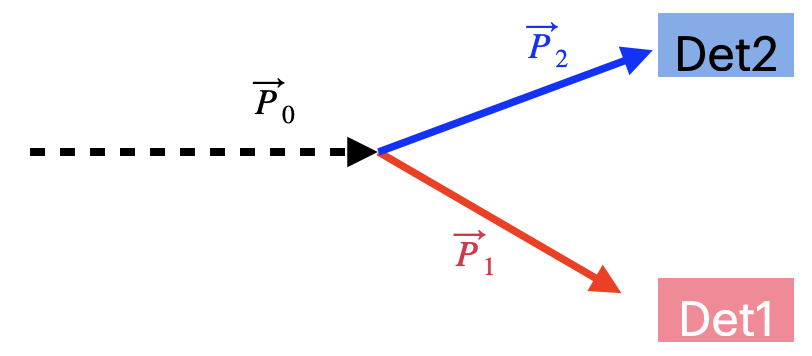
\includegraphics[width=.9\textwidth]{TwoBodyDecay}
		\end{figure}
	}{
	\begin{block}{}
		\large
		Assume a beam with momentum $\vec P^-$ decays into $\vec P_1$ and $\vec P_2$. Measured momentum are smeared due to detector resolution, leading to unbalance in the momentum conservation.
		\begin{align}
			\vec P_{0}=\vec P_{1}+\vec P_{2};\quad \vec P_{1,meas} + \vec P_{2,meas}\neq \vec P_{0} 
		\end{align}
		
	\end{block}
	}
	\begin{block}{}
		\large
	We can define the $\chi^2$ to quantitatively represent our measurement error. However, we can't derive meaningful expressions from this $\chi^2$. 
	\begin{align}
		\chi^2= \frac{(P_{1}-P_{1,meas})^2}{\sigma_1^2}+\frac{(P_{2}-P_{2,meas})^2}{\sigma_2^2}\label{chi2}
	\end{align}
	\end{block}
\end{frame}
\begin{frame}{Constrained Optimization with The Lagrange Multiplier}
	\begin{block}{}
		By incorporating the \textit{Kinematic Constraints}, specifically \textit{momentum conservation}, we involve additional knowledge to \eqref{chi2}. This is known as the \textit{Lagrange Multiplier}
		\begin{align}
			\chi^2= \frac{(P_{1,KF}-P_{1,meas})^2}{\sigma_1^2}+\frac{(P_{2,KF}-P_{2,meas})^2}{\sigma_2^2} + 2\mathbf{\lambda(P_{1,KF}+P_{2,KF}-P_0)}\label{LagMulti}
		\end{align} 
		Now we have meaningful expressions to minimize $\chi^2$, hence get better estimations for the measurement.
		\begin{align}
			\frac{1}{2}\pdf{\chi2}{P_{1,KF}}&=\frac{(P_{1,KF}-P_{1,meas})}{\sigma_1^2}+\lambda=0\label{dxd1}\\
			\frac{1}{2}\pdf{\chi2}{P_{2,KF}}&=\frac{(P_{2,KF}-P_{2,meas})}{\sigma_2^2}+\lambda=0\label{dxd2}
			\\
			\frac{1}{2}\pdf{\chi2}{\lambda}&=(P_{1,KF}+P_{2,KF}-P_0)=0\label{dxdl}
		\end{align}
	\end{block}
\end{frame}
\begin{frame}{Why Better Resolution?}
	\begin{block}{}
		By solving the equations \ref{dxd1},\ref{dxd2},\ref{dxdl} and defining $\delta_i = P_{i,meas} - P_i$, we obtain the following expressions:
		\begin{align}
			\lambda&=\frac{P_{1,meas}+P_{2,meas}-P_0}{\sigma_1^2+\sigma_2^2} = \frac{\delta_1 + \delta_2}{\sigma_1^2+\sigma_2^2}\\
			P_{1,KF}&=P_{1,meas}-\sigma_1^2\lambda\\
			P_{2,KF}&=P_{2,meas}-\sigma_2^2\lambda
		\end{align}
		\begin{align}
		<P_{1,KF}-P_{1}>& =<P_{1,KF}-P_{1,meas}+\delta_{1}>  = <-\sigma_1^2\lambda+\delta_1>\nonumber\\
		&=<\frac{-\sigma_1^2}{\sigma_1^2+\sigma_2^2}(\delta_{1}+\delta_{2})+\delta_1>=<\frac{\sigma_2^2\delta_1 -\sigma_1^2\delta_2}{\sigma_1^2+\sigma_2^2}> \\
		\sigma_{1,KF}^2 &= <(P_{1,KF}- P_1)^2> =\frac{\sigma_2^4\cancelto{\sigma_1^2}{<\delta_1^2>}+\sigma_1^4\cancelto{\sigma_2^2}{<\delta_2^2>}}{(\sigma_1^2+\sigma_2^2)^2} = \frac{\sigma_1^2\sigma_2^2}{\sigma_1^2+\sigma_2^2}<\sigma_1^2
	\end{align}
	\end{block}
\end{frame}
\begin{frame}{The Covariance After Kinematic Fit}
	\begin{block}{}
		\begin{align}
			cov(P_{1},P_{2})_{KF}& = <\delta_{1,KF}\delta_{2,KF}> = <(\delta_1 -\sigma_1^2\lambda)(\delta_2-\sigma_2^2\lambda)> \nonumber\\
			&= \sigma_1^2\sigma_2^2\cancelto{\frac{1}{\sigma_1^2+\sigma_2^2}}{<\lambda^2>}\quad -\quad \frac{\sigma_1^2<\delta_2^2>+\sigma_2^2<\delta_1^2>}{\sigma_1^2+\sigma_2^2} =-\frac{\sigma_1^2\sigma_2^2}{\sigma_1^2+\sigma_2^2}
		\end{align}
		\begin{align}
			V=\begin{pmatrix}
				\sigma_1^2&0\\
				0&\sigma_2^2
			\end{pmatrix}\to V_{KF} =
			\begin{pmatrix}
\frac{\sigma_1^2\sigma_2^2}{\sigma_1^2+\sigma_2^2}&-\frac{\sigma_1^2\sigma_2^2}{\sigma_1^2+\sigma_2^2}\\
-\frac{\sigma_1^2\sigma_2^2}{\sigma_1^2+\sigma_2^2}&\frac{\sigma_1^2\sigma_2^2}{\sigma_1^2+\sigma_2^2}
			\end{pmatrix}
		\end{align}
		\begin{itemize}
			\item Improved momentum resolution
			\item Negative correlation between $P_1$ and $P_2$
		\end{itemize}
	\end{block}
\end{frame}
\begin{frame}{Generalization to Multi-Variables}
	\begin{block}{}
		Assume that we have a set of measured data $\mathbf{m^0}$, unknown parameters $\mathbf {u^0}$ and constraints $\mathbf f^0$.
		\begin{align}
			\mathbf {m^0} =\{m_1^0,m_2^0\ldots m_N^0\};\quad \mathbf {u^0} =\{u_1^0,u_2^0\ldots u_J^0\}\nonumber\\
			\mathbf f =\{f_1(m_1^0,m_2^0,\ldots m_N^0,u_1^0,u_2^0,\ldots u_N^0),f_2^0,\ldots f_K^0\}
		\end{align}
		 Let $\mathbf m^0$ denote our initial measured data, and $\mathbf m$ represent the 'guess' of the data in each iterative step, just alike $P_{KF}$s in the previous example. Equation \eqref{LagMulti} is generalized to:
		\begin{align}
			\chi^2(\mathbf{m}) = (\mathbf{m}^0-\mathbf{m})^\dagger V^{-1}(\mathbf{m}^0-\mathbf{m})+2\mathbf\lambda^\dagger \mathbf {f}(\mathbf{m,u}).\label{KFChi2}
		\end{align}
		Here, the Lagrange multiplier $\mathbf \lambda =\{\lambda_1,\lambda_2,\ldots\lambda_K\}$ is not just a number but a column vector with k elements, corresponding to each kinematic constraint in $\mathbf f$. 
	\end{block}
\end{frame}

\begin{frame}{$\chi^2$ Minimization}
	\begin{block}{}
		We want to solve the equation
		\begin{align}
			\vec \nabla \chi^2 =0
		\end{align}
		to obtain the minimized state. The differential term are listed within three groups.
		\begin{align}
			\nabla_{\mathbf m} &= -2 V^{-1}(\mathbf m^0)(\mathbf m^0-\mathbf m) + 2 \mathbf F_\mathbf m^\dagger(\mathbf{m,u})\mathbf\lambda=0\label{GradM}\\
			\nabla_{\mathbf u} &= 2\mathbf F_\mathbf u^\dagger(\mathbf{m,u})\mathbf \lambda =0\label{GradU}\\
			\nabla_{\mathbf \lambda}& = \mathbf f(\mathbf{m,u})\label{GradL}.
		\end{align}
		Here, the subscripts denote partial derivatives. i.e. ($(\mathbf {F}_m)_{ki}\equiv\pdf {f_k}{m_i}$).
	\end{block}
	\begin{block}{User Should Define...}
		\begin{table}
			\begin{tabular}{c|c|c|c|c}
				$\mathbf{m}$&$\mathbf{u}$&$\mathbf{f}$&$\mathbf{V}$&$\mathbf{F_m},\mathbf{F_u}$\\\hline
				Measured Data&Unknown parameters&Constraints&Covariance Matrix&Derivatives
			\end{tabular}
		\end{table}
	\end{block}
\end{frame}
\begin{frame}{Pull distribution}
	\begin{block}{}
		A bias or resolution miss-estimation is revealed by observing the \textit{Pull distribution} of each measurements. However, we cannot evaluate the 'true' value of measurement, hence pull for the real data is not accessible. Instead, from the the residual $\epsilon = m-m^0$ and its variance $V(\epsilon)$, we observe the pull(of the residual) as :
		\begin{align}
			P(\epsilon) = \epsilon/\sqrt{V(\epsilon)}\label{Pull}
		\end{align}
		and
		\begin{align}
			V(\epsilon) \equiv V(m)+ V(m^0) - 2 Cov(m,m^0).\label{Ve}
		\end{align}
		The variance of the fitted variables, $V(m)$, is evaluated as
		\begin{align}
			V(m) = J_{m,m^0}V(m^0) J^\dagger_{m,m^0} 
		\end{align}
		 where $J_{m,m^0}$ is the Jacobian for $m$ and $m^0$. Detailed calculations are provided in the appendix. 
	\end{block}
\end{frame} 
\section{Example: Mass-Constraint Fit}
\begin{frame}{Example: $\Lambda\to p\pi$, Defining Variables and Constraints}
	\begin{block}{}
		Assume a decay of $\Lambda\to p\pi^-$. We define the measurements and unknowns as:
		\begin{align}
			\mathbf{m}=\{P_p,\theta_p,\phi_p,P_\pi,\theta_\pi,\phi_\pi\};\quad\mathbf{u} = \{P_\Lambda,\theta_\Lambda,\phi_\Lambda\}
		\end{align}
		Then we define the energy-momentum constraint equation as:
		\begin{align}
			\begin{pmatrix}
				f_1\\f_2\\f_3\\f_4
			\end{pmatrix}=
			\begin{pmatrix}
				-P_\Lambda\sin\theta_\Lambda\cos\phi_\Lambda+P_p\sin\theta_p\cos\phi_p+P_\pi\sin\theta_\pi\cos\phi_\pi\\
				-P_\Lambda\sin\theta_\Lambda\sin\phi_\Lambda+P_p\sin\theta_p\sin\phi_p+P_\pi\sin\theta_\pi\sin\phi_\pi\\
				-P_\Lambda\cos\theta_\Lambda+P_p\cos\theta_p+p_\pi\cos\theta_\pi\\
				-\sqrt{P_\Lambda^2+m_\Lambda^2}+\sqrt{P_p^2+m_p^2}+\sqrt{P_\pi^2+m_\pi^2}
			\end{pmatrix}.\label{FMat}
		\end{align}
		where the mass constraint is naturally implemented in energy term.
		
		Since we have 3 unmeasured variable with 4 kinematical constraints, this is a 4-3 = 1-Constrained fit.
	\end{block}
\end{frame}
\begin{frame}{Example: $\Lambda\to p\pi$, The Derivatives}
	\begin{block}{}
		 We get $\mathbf{F_u}$ and $\mathbf{F_m}$ as
		\begin{align}
			\mathbf{F_u}=
			\begin{pmatrix}
				\pdf{f_1}{P_\Lambda}&\pdf{f_1}{\theta_\Lambda}&\pdf{f_1}{\phi_\Lambda}\\
				\pdf{f_2}{P_\Lambda}&\pdf{f_2}{\theta_\Lambda}&\pdf{f_2}{\phi_\Lambda}\\
				\pdf{f_3}{P_\Lambda}&\pdf{f_3}{\theta_\Lambda}&\pdf{f_3}{\phi_\Lambda}\\
				\pdf{f_4}{P_\Lambda}&\pdf{f_4}{\theta_\Lambda}&\pdf{f_4}{\phi_\Lambda}
			\end{pmatrix};\quad \mathbf{F_m}=\begin{pmatrix}
				\pdf{f_1}{P_p} &\cdots&\pdf{f_1}{\phi_\pi} \\
				\pdf{f_2}{P_p} &\cdots&\pdf{f_2}{\phi_\pi}\\
				\pdf{f_3}{P_p} &\cdots&\pdf{f_3}{\phi_\pi}\\
				\pdf{f_4}{P_p} &\cdots&\pdf{f_4}{\phi_\pi}
			\end{pmatrix}
		\end{align}
		We have all the matrices to calculate in each step. By applying an appropriate variance matrix and employing $\chi^2$ selection criteria, we can do kinematic fit for the particles.
	\end{block}
\end{frame}
\begin{frame}{Example: $\Xi\to \Lambda\pi$, $\Lambda\to p\pi$}
	\begin{block}{}
		We require two mass constraints for $\Xi\to \Lambda\pi;\quad \Lambda\to p\pi$. In this case, careful considerations on the selection of variables. We will select
		\begin{align}
			\mathbf{u} = \{P_\Xi,\theta_\Xi,\phi_\Xi\};\quad \mathbf{m}=\{P_p,\theta_p,\phi_p,P_\pi,\theta_\pi,\phi_\pi\}
		\end{align}
		and define five constraints as:
		\begin{align}
			\begin{pmatrix}
				f_1\\f_2\\f_3\\f_4\\f_5
			\end{pmatrix}=
			\begin{pmatrix}
				-P_{\Xi,x}+P_{p,x}+P_{{\pi_\Lambda},x}+P_{{\pi_\Xi},x}\\
				-P_{\Xi,y}+P_{p,y}+P_{{\pi_\Lambda},y}+P_{{\pi_\Xi},y}\\
				-P_{\Xi,z}+P_{p,z}+P_{{\pi_\Lambda},z}+P_{{\pi_\Xi},z}\\
				-E_\Lambda +E_p+E_{\pi_\Lambda}\\
				-E_\Xi +E_p+E_{\pi_\Lambda}+E_{\pi_\Xi}
			\end{pmatrix}.
		\end{align}
			$\Lambda$ variables($\{P_\Lambda,\theta_\Lambda,\phi_\Lambda\}$) are not selected in $\mathbf u$ to reduce matrix dimension.
			That is, \textbf{we don't have explicit terms} related to $\vec P_\Lambda$, i.e.  $-P_{\Lambda,x}+P_{p,x}+P_{{\pi_\Lambda},x}$ etc., because $\vec P_\Lambda$ are neither unmeasured nor measured variables in our choice of parameters.  
	\end{block}
\end{frame}
\begin{frame}{Kinematics Restoration}
	\tcl{8}{8}{
		\begin{figure}
			\begin{picture}(200,150)
				\put(-10,0){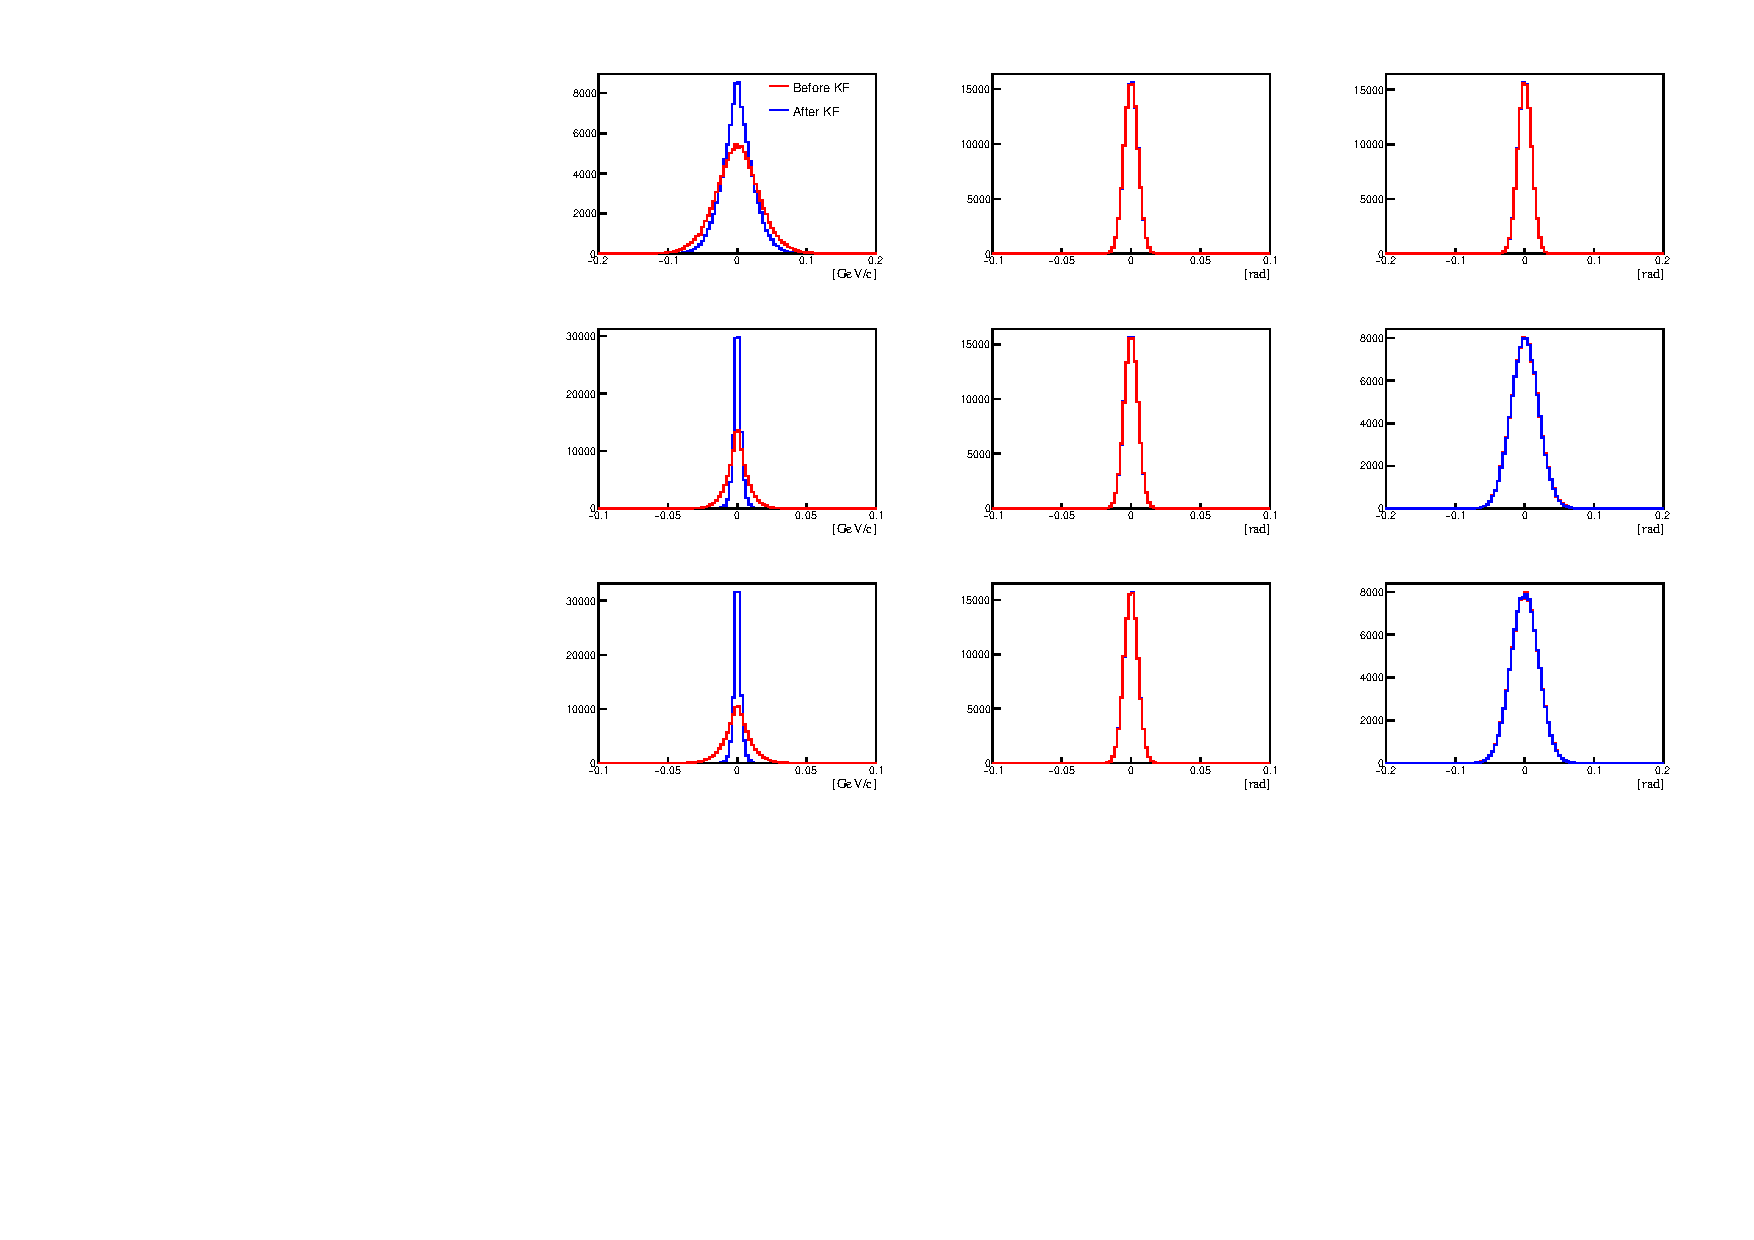
\includegraphics[width=.95\textwidth]{Xi_cKF1}}
				\put(20,40){\rotatebox{15}{\Huge\textcolor{tubsgray20}{ToySimulation}}}
			\end{picture}
		\end{figure}
	}{
	\begin{figure}
		\begin{picture}(200,150)
			\put(-10,0){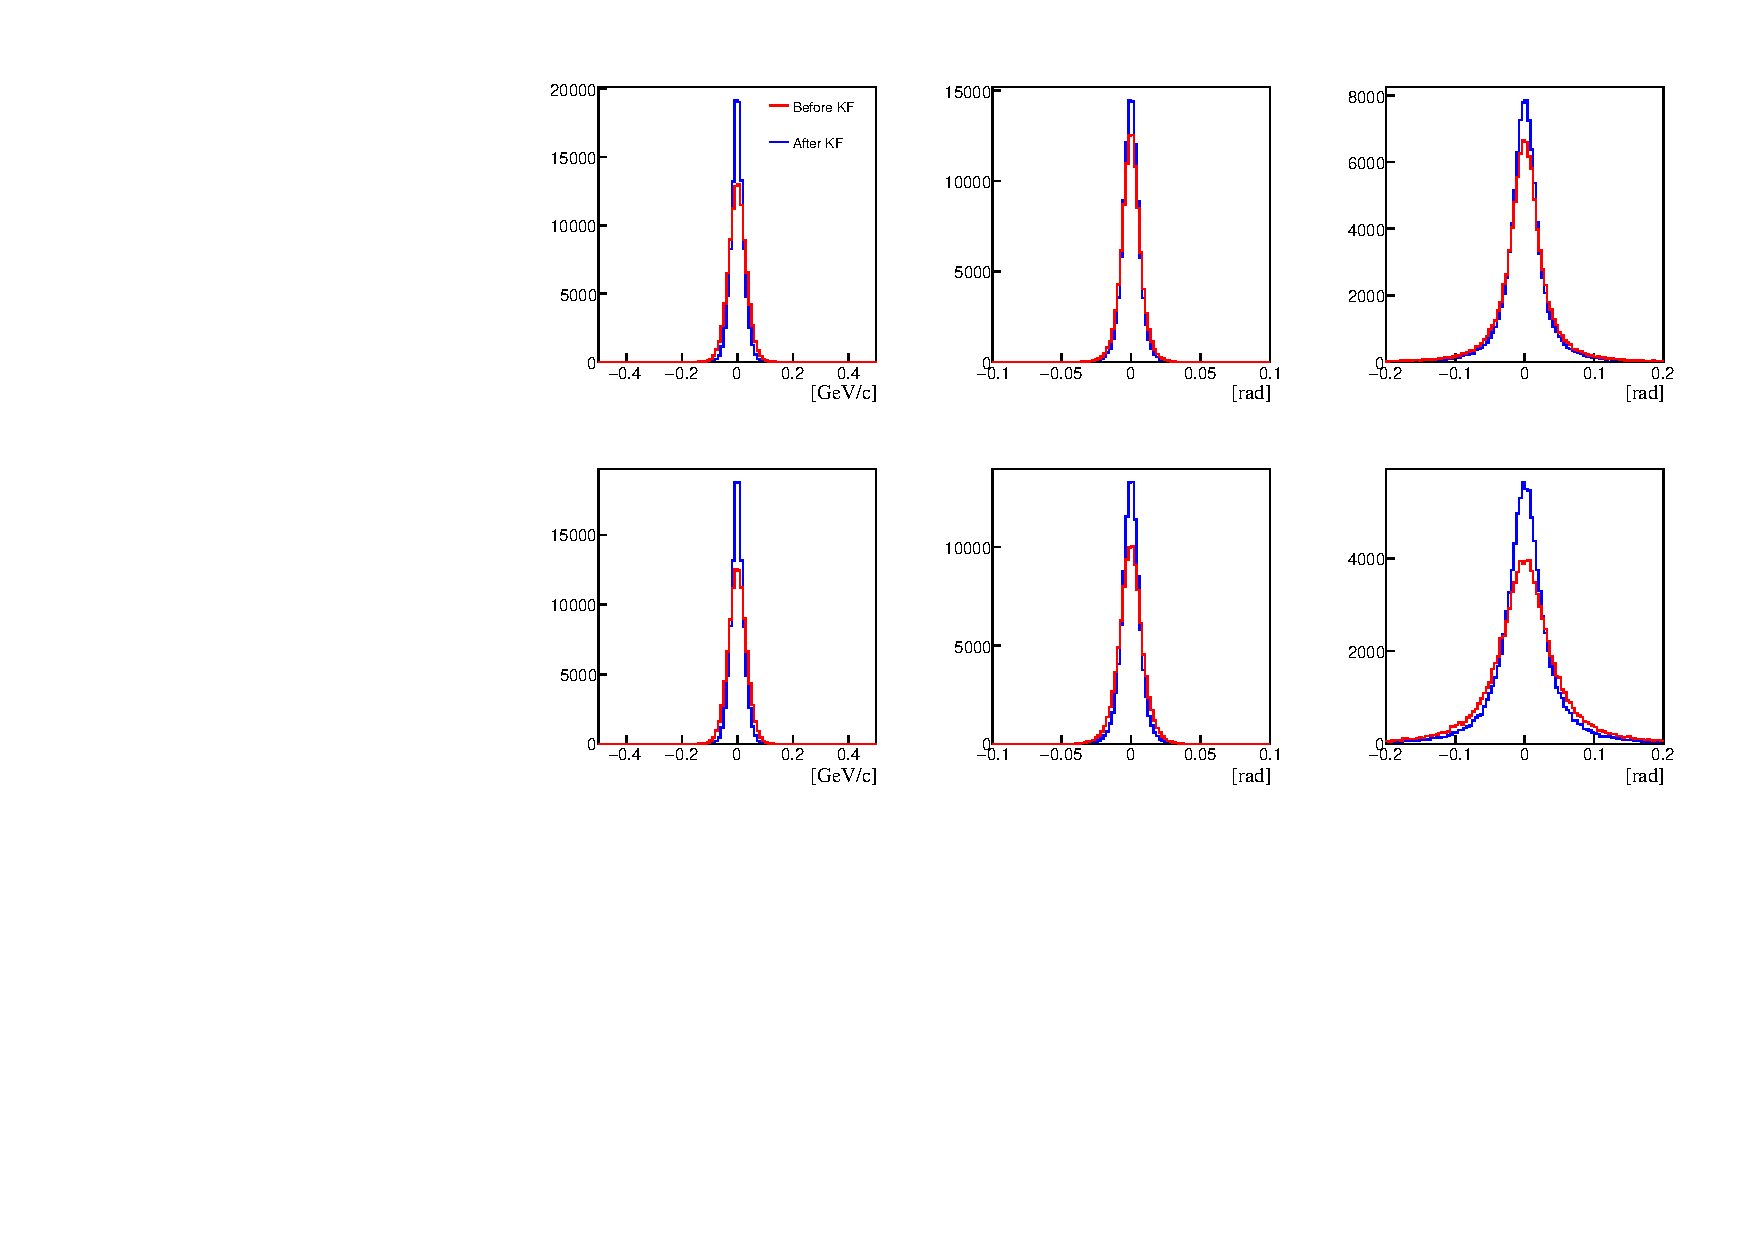
\includegraphics[width=.95\textwidth]{Xi_cKF2}}
			\put(20,40){\rotatebox{15}{\Huge\textcolor{tubsgray20}{ToySimulation}}}
		\end{picture}
	\end{figure}
	}
\end{frame}
\begin{frame}{Pull Distribution}
	\tcl{8}{8}{
	\begin{figure}
		\begin{picture}(200,150)
			\put(-10,0){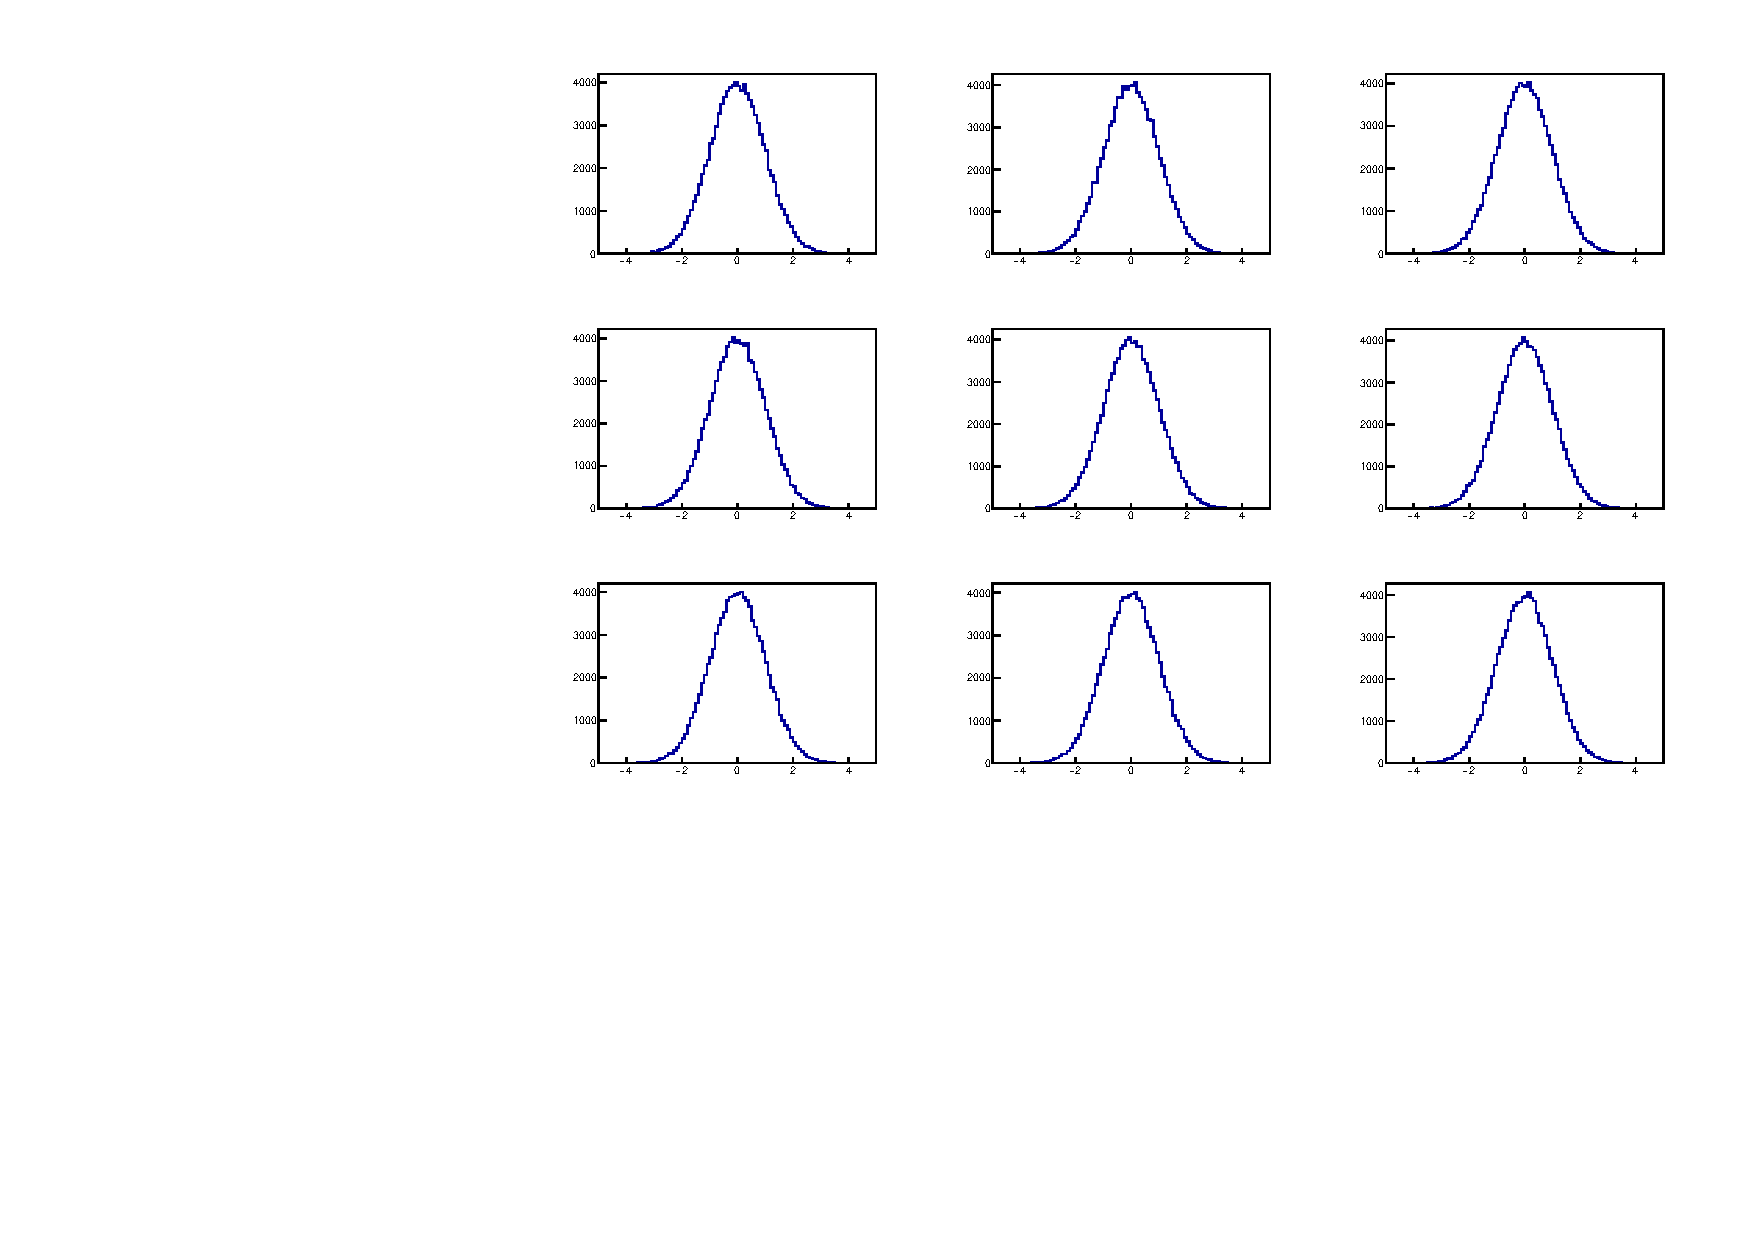
\includegraphics[width=.95\textwidth]{Xi_cKF4}}
			\put(20,40){\rotatebox{15}{\Huge\textcolor{tubsgray20}{ToySimulation}}}
		\end{picture}
	\end{figure}
}{
\begin{block}{}
		\begin{align}
		P(X) = \frac{X_{KF} - X_0}{\sqrt{V(X_{KF} - X_{0})}}
	\end{align}
	\begin{itemize}
		\item Pull distribution shows the normalized amount of parameter adjustment.
		\item Gaussian distribution with $\sigma=1$  implies good understandings in covariance of the measurement.
		\item In practice, resolution can be iteratively scaled by 1./ pull width
	\end{itemize}
\end{block}
}
\end{frame}
\begin{frame}{$\Xi^*(1530)\to \Xi \pi^0$ and $\Xi^*(1530)\to \Xi^0 \pi^-$ Separation}
	\begin{block}{}
		\begin{figure}
			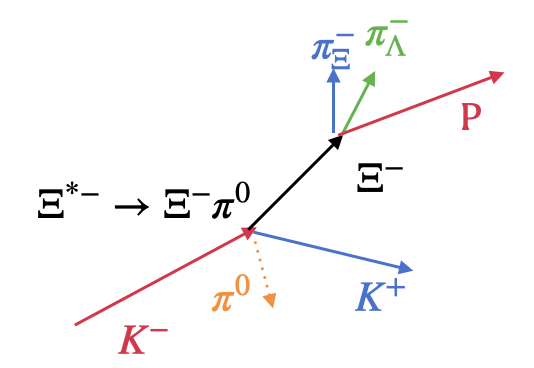
\includegraphics[height = 40mm]{MissingXiStar}
			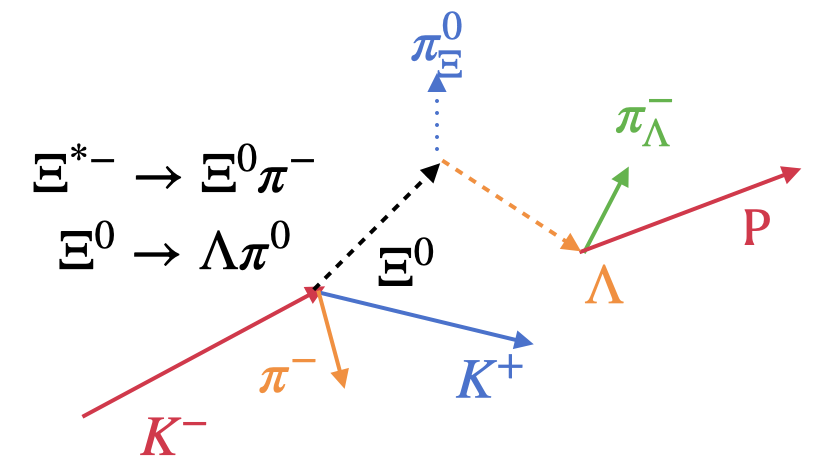
\includegraphics[height = 40mm]{MissingXiStarXi0}
		\end{figure}
		\begin{itemize}
			\item{Two decay channel of $\Xi^*$ share the same decay product.}
			\item{Separation criteria should be defined to distinguish combinatorial backgrounds.}
			\item{Kinematic Fit result can provide another selection criteria based on Kinematics.}
		\end{itemize}
	\end{block}
\end{frame}
\begin{frame}{Invariant Mass}
	\begin{block}{}
		\begin{figure}
			\begin{picture}(400,200)
				\put(20,0){
					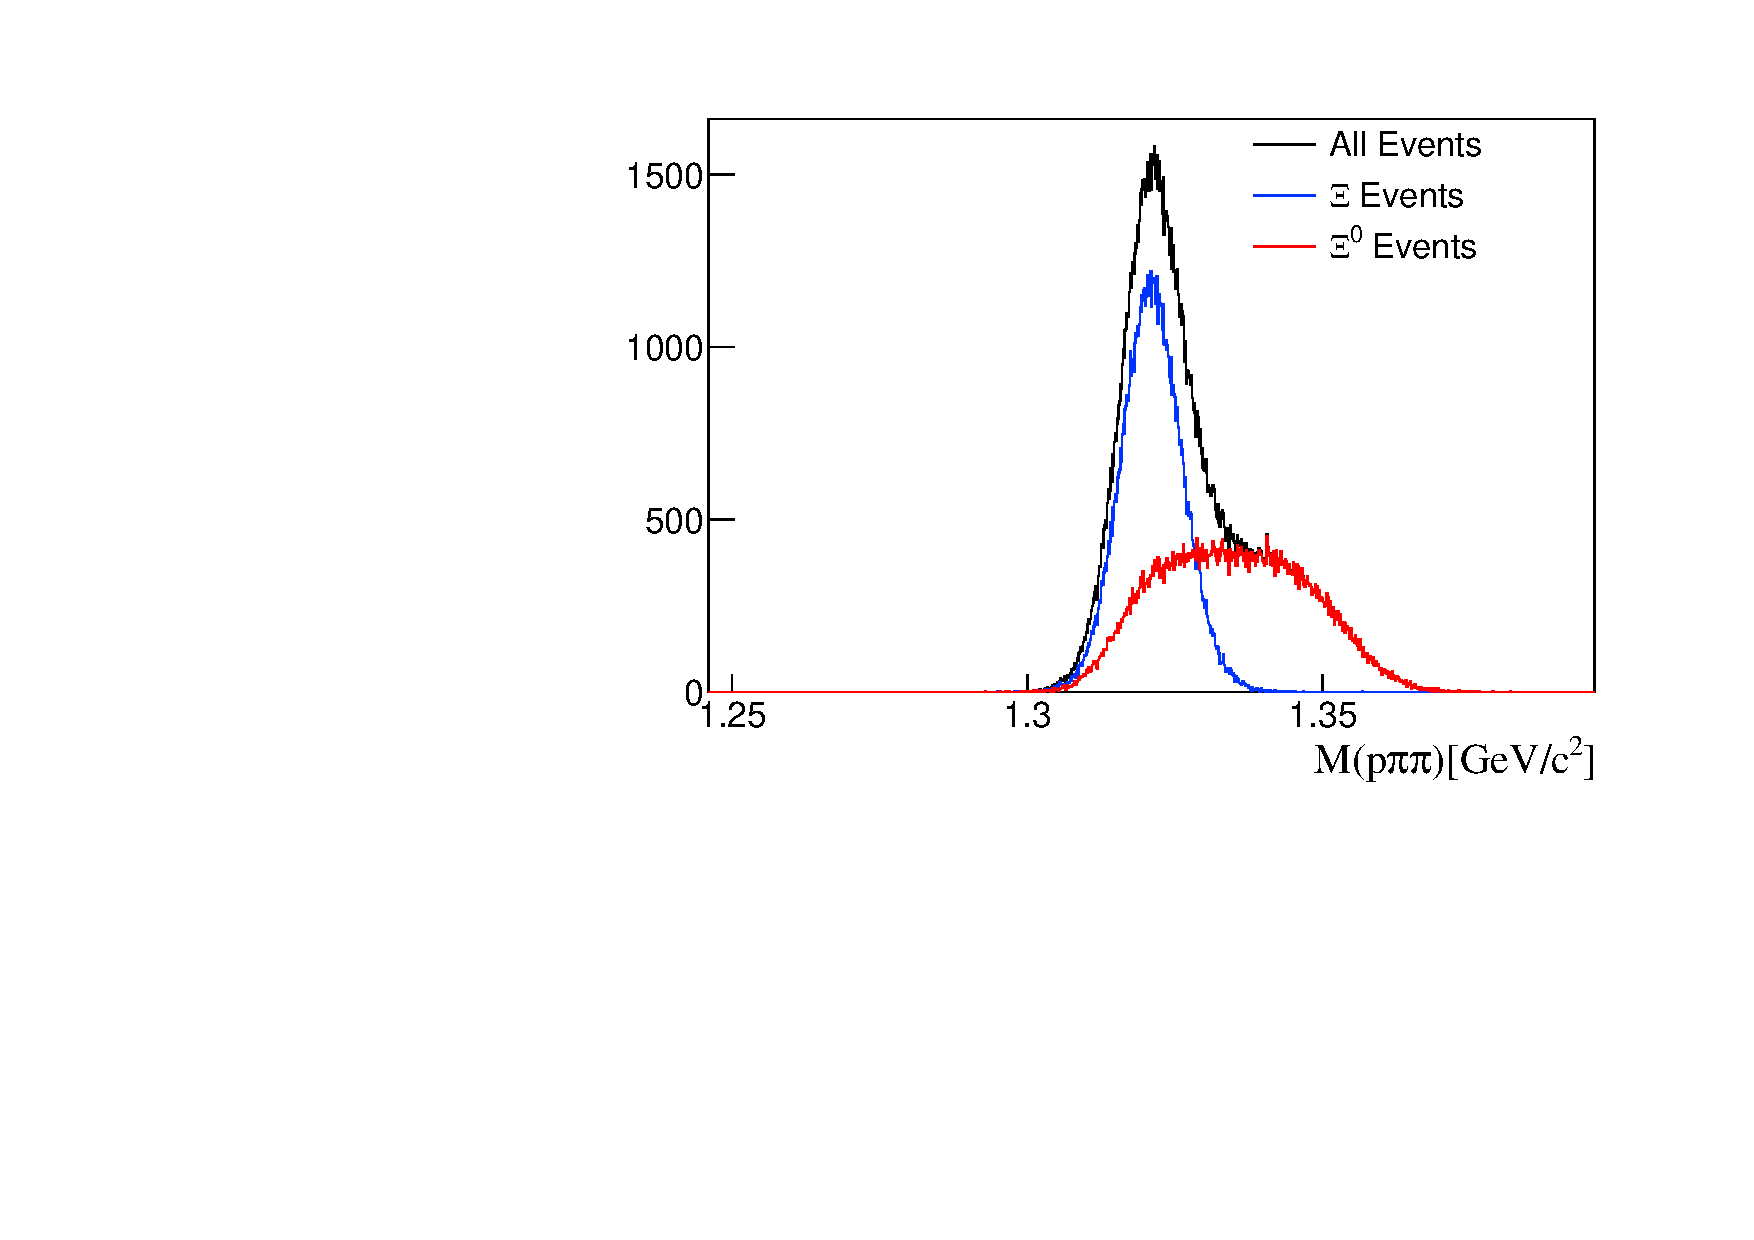
\includegraphics[width = .8\textwidth]{c_imxi}
					\put(-200,80){\rotatebox{15}{\Huge\textcolor{tubsgray20}{ToySimulation}}}
				}
			\end{picture}			
		\end{figure}
	\end{block}
\end{frame}
\begin{frame}{Mass Window Selection}
	\begin{block}{}
				\begin{figure}
			\begin{picture}(400,200)
				\put(20,0){
					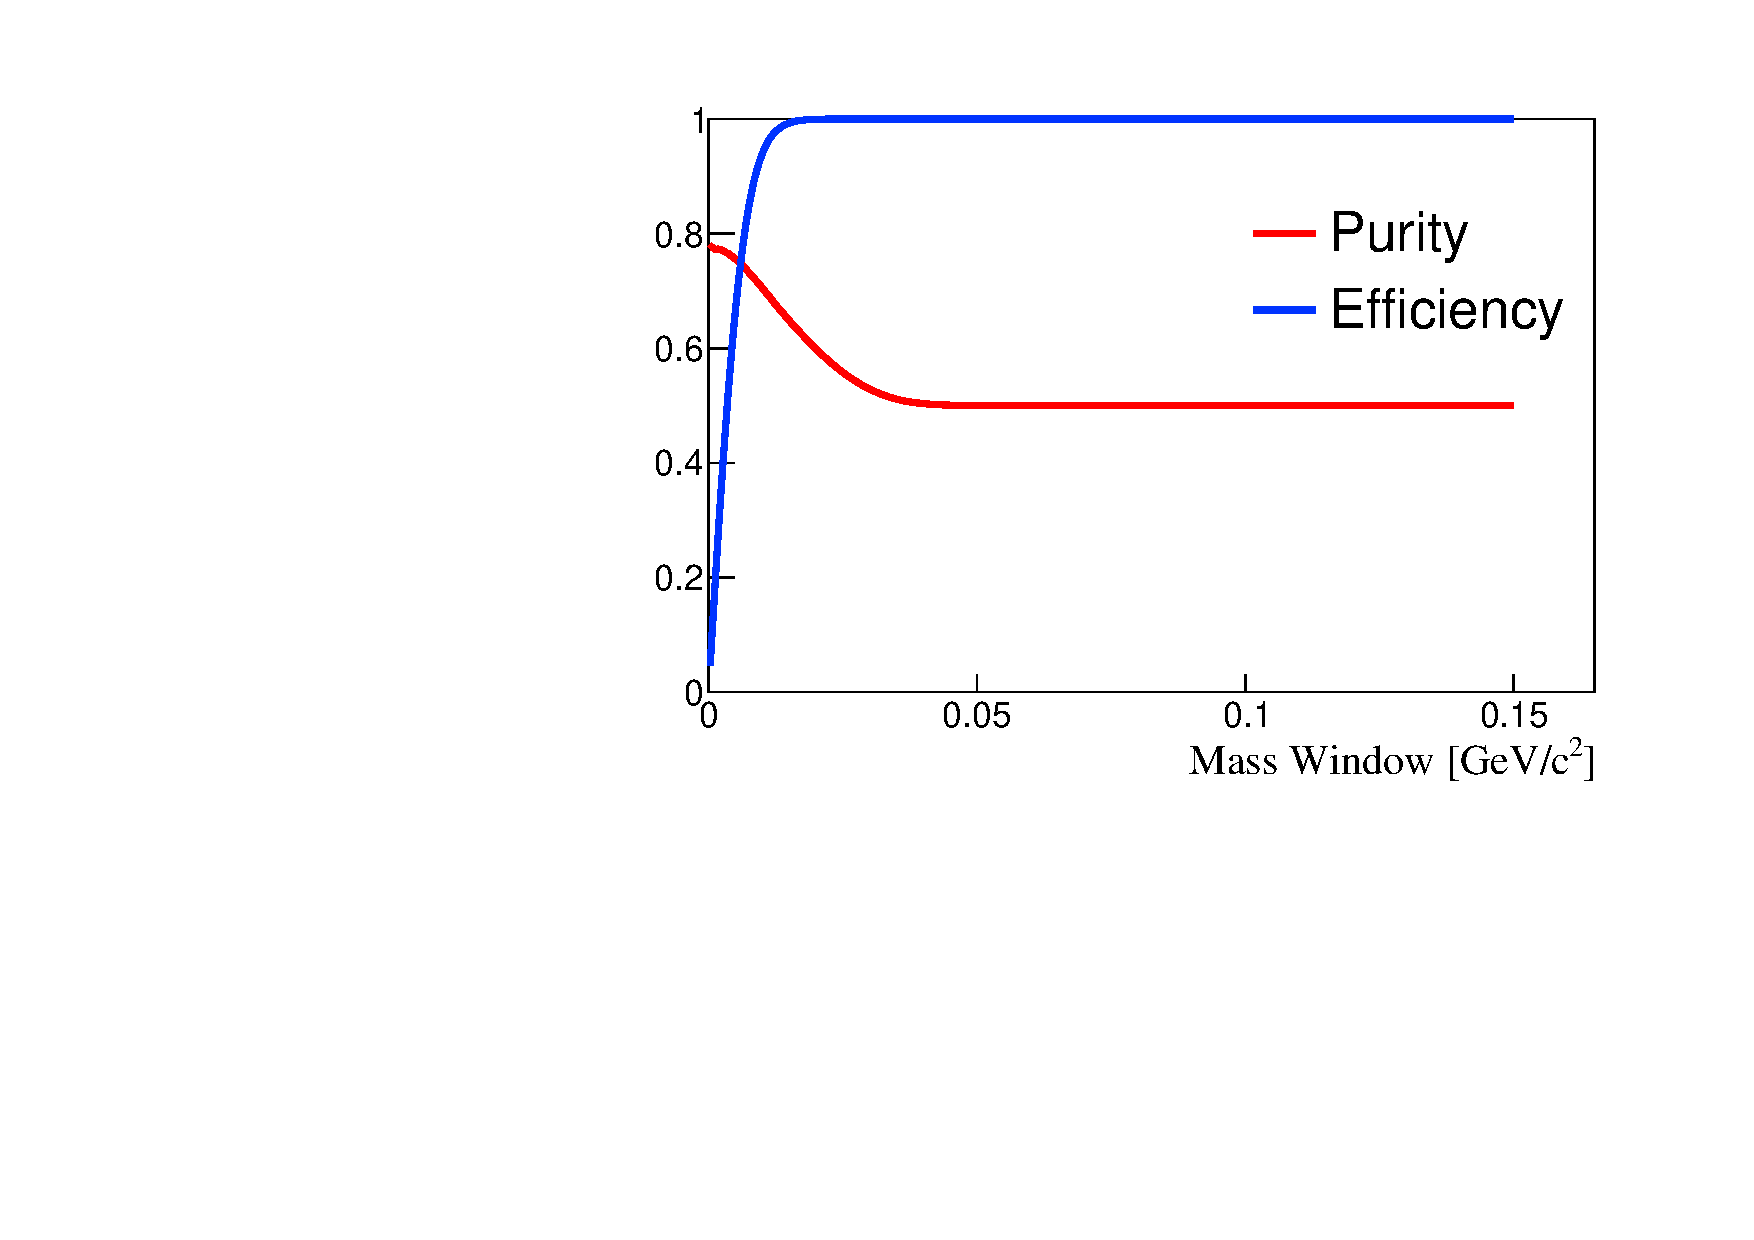
\includegraphics[width = .8\textwidth]{c_mass}
					\put(-200,80){\rotatebox{15}{\Huge\textcolor{tubsgray20}{ToySimulation}}}
				}
			\end{picture}			
		\end{figure}		
	\end{block}
\end{frame}
\begin{frame}{The P-value}
	\begin{block}{}
				\begin{figure}
			\begin{picture}(400,200)
				\put(20,0){
					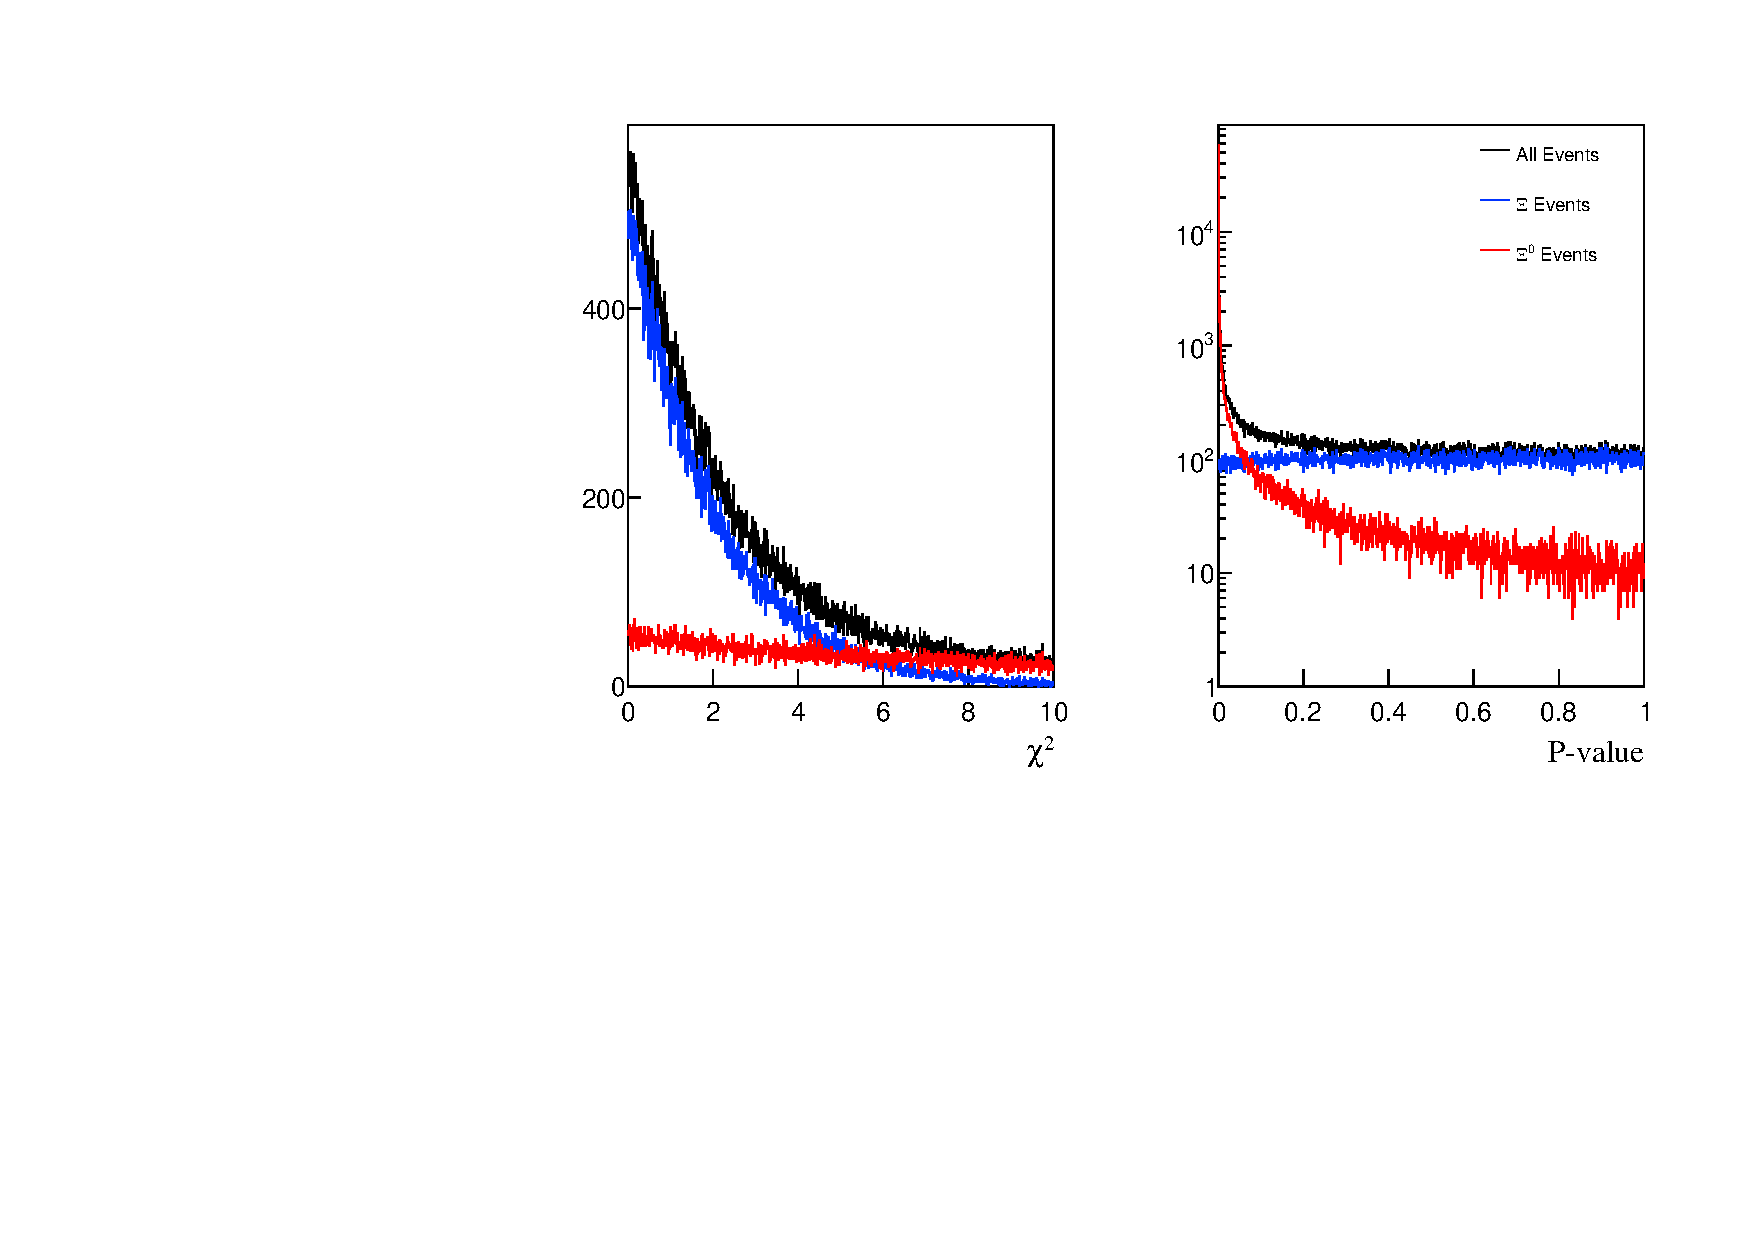
\includegraphics[width = .8\textwidth]{c_sum}
					\put(-200,80){\rotatebox{15}{\Huge\textcolor{tubsgray20}{ToySimulation}}}
				}
			\end{picture}			
		\end{figure}
		
	\end{block}
\end{frame}
\begin{frame}{P-value Selection}
	\begin{block}{}
				\begin{figure}
			\begin{picture}(400,200)
				\put(20,0){
					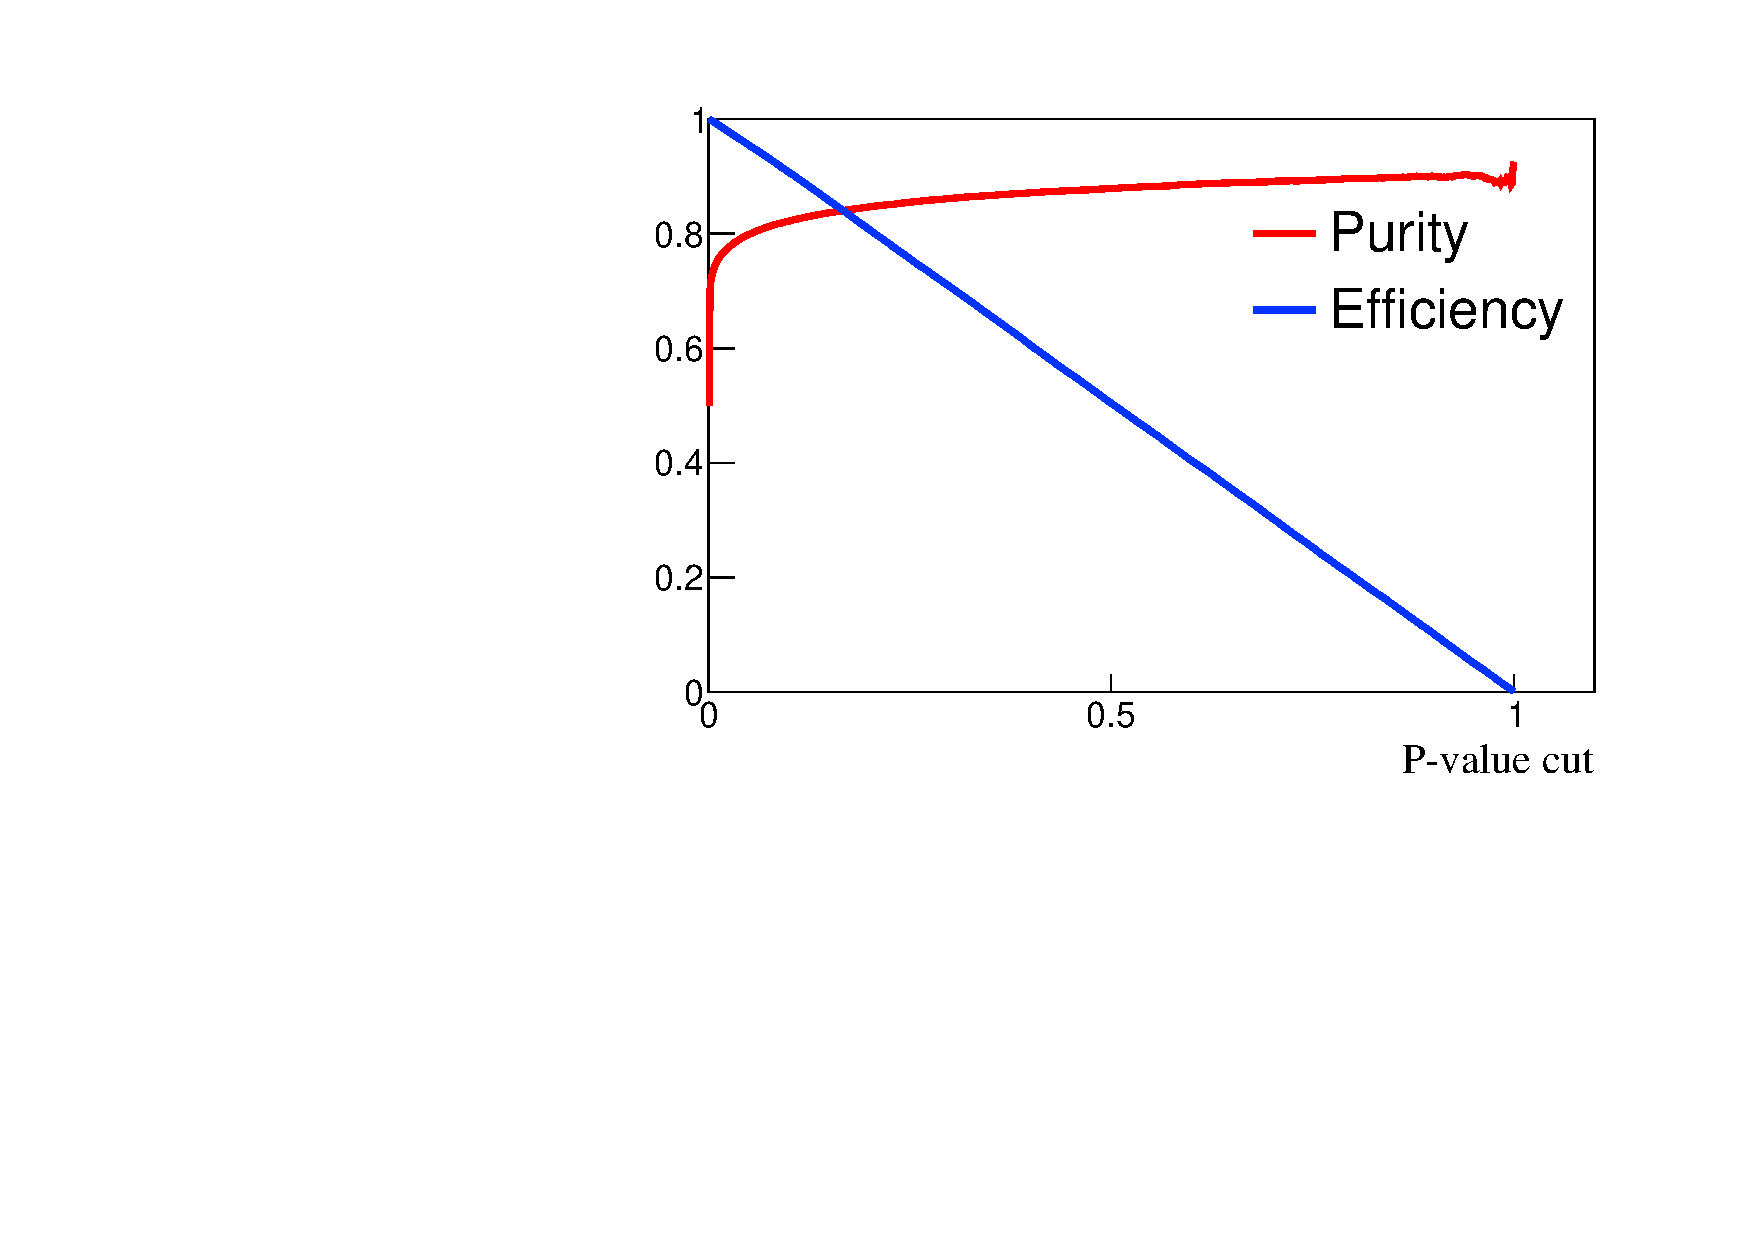
\includegraphics[width = .8\textwidth]{c_pval}
					\put(-200,80){\rotatebox{15}{\Huge\textcolor{tubsgray20}{ToySimulation}}}
				}
			\end{picture}			
		\end{figure}
		
	\end{block}
\end{frame}
\begin{frame}{P-value vs Invariant Mass}
	\begin{block}{}
				\begin{figure}
			\begin{picture}(400,200)
				\put(20,0){
					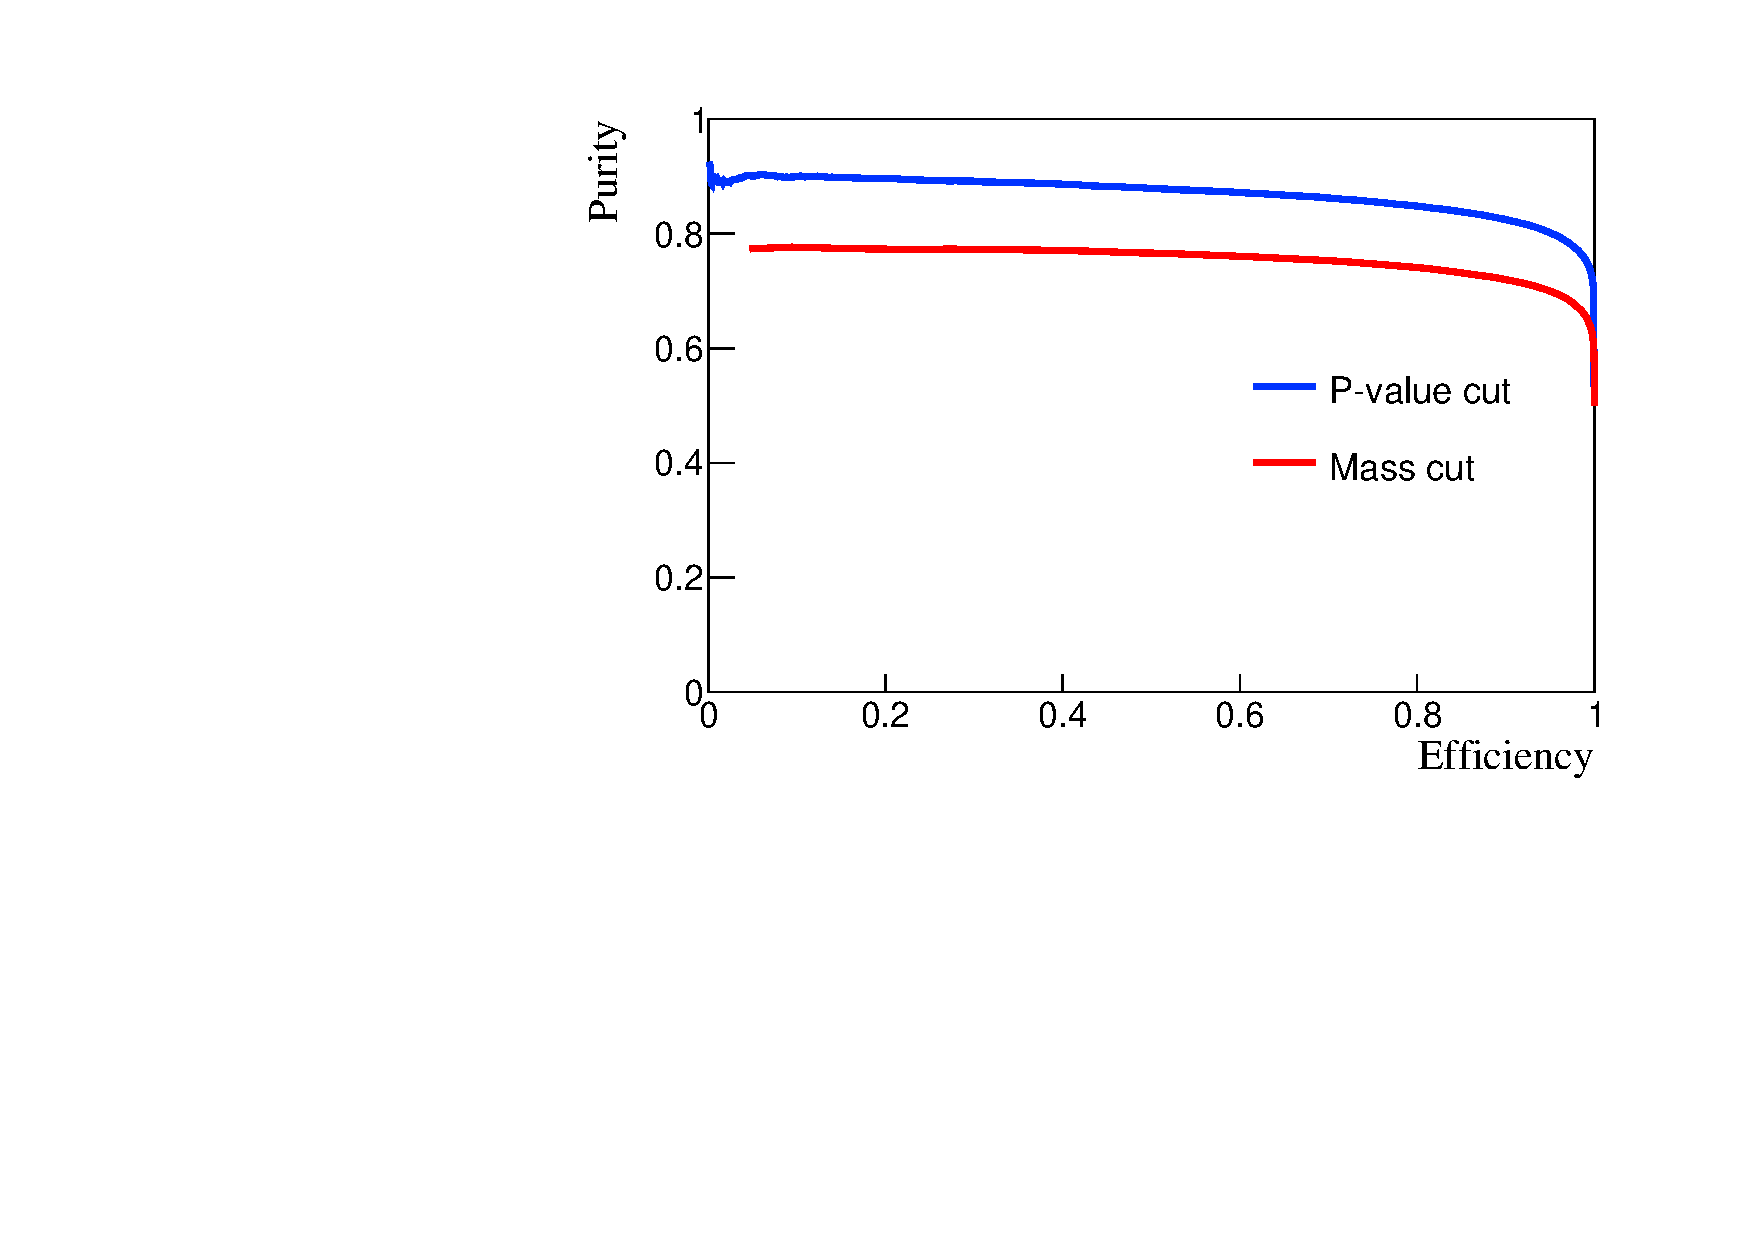
\includegraphics[width = .8\textwidth]{c_eff_pur}
					\put(-200,80){\rotatebox{15}{\Huge\textcolor{tubsgray20}{ToySimulation}}}
				}
			\end{picture}			
		\end{figure}
		
	\end{block}	
\end{frame}
\begin{frame}{Example: MassVertex-Constraint Fit}
	\begin{block}{}
		To be Updated..
	\end{block}
\end{frame}
\section{Applications: $\Xi $ decay at J-PARC}
\begin{frame}{$p(K^-,K^+)X$ at J-PARC E42}
	\tcl{5}{10}{
	\begin{block}{}
		\begin{figure}
			\begin{picture}(100,200)
				\put(20,0){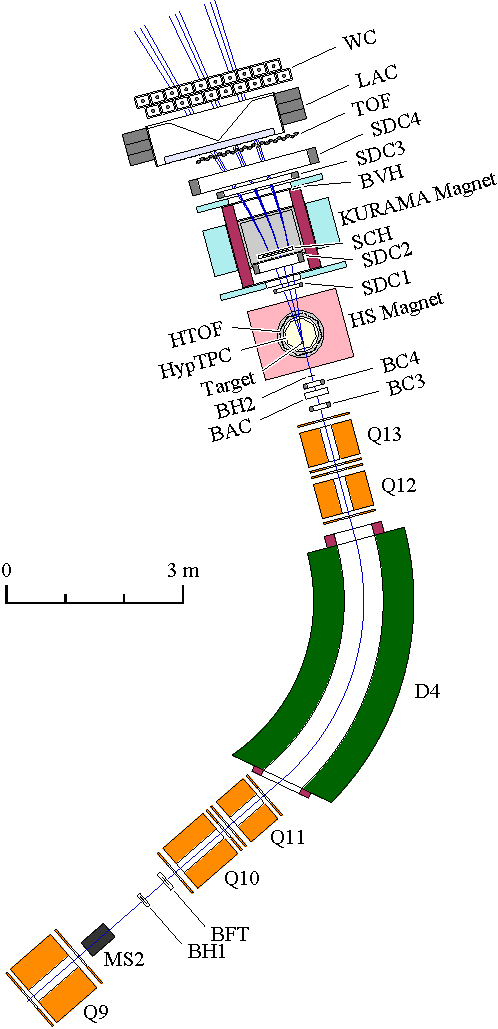
\includegraphics[width = 3.3 cm]{K18}}
			\end{picture}
		\end{figure}
	\end{block}
	}{
	\begin{figure}
		\begin{picture}(200,200)
			\put(0,0){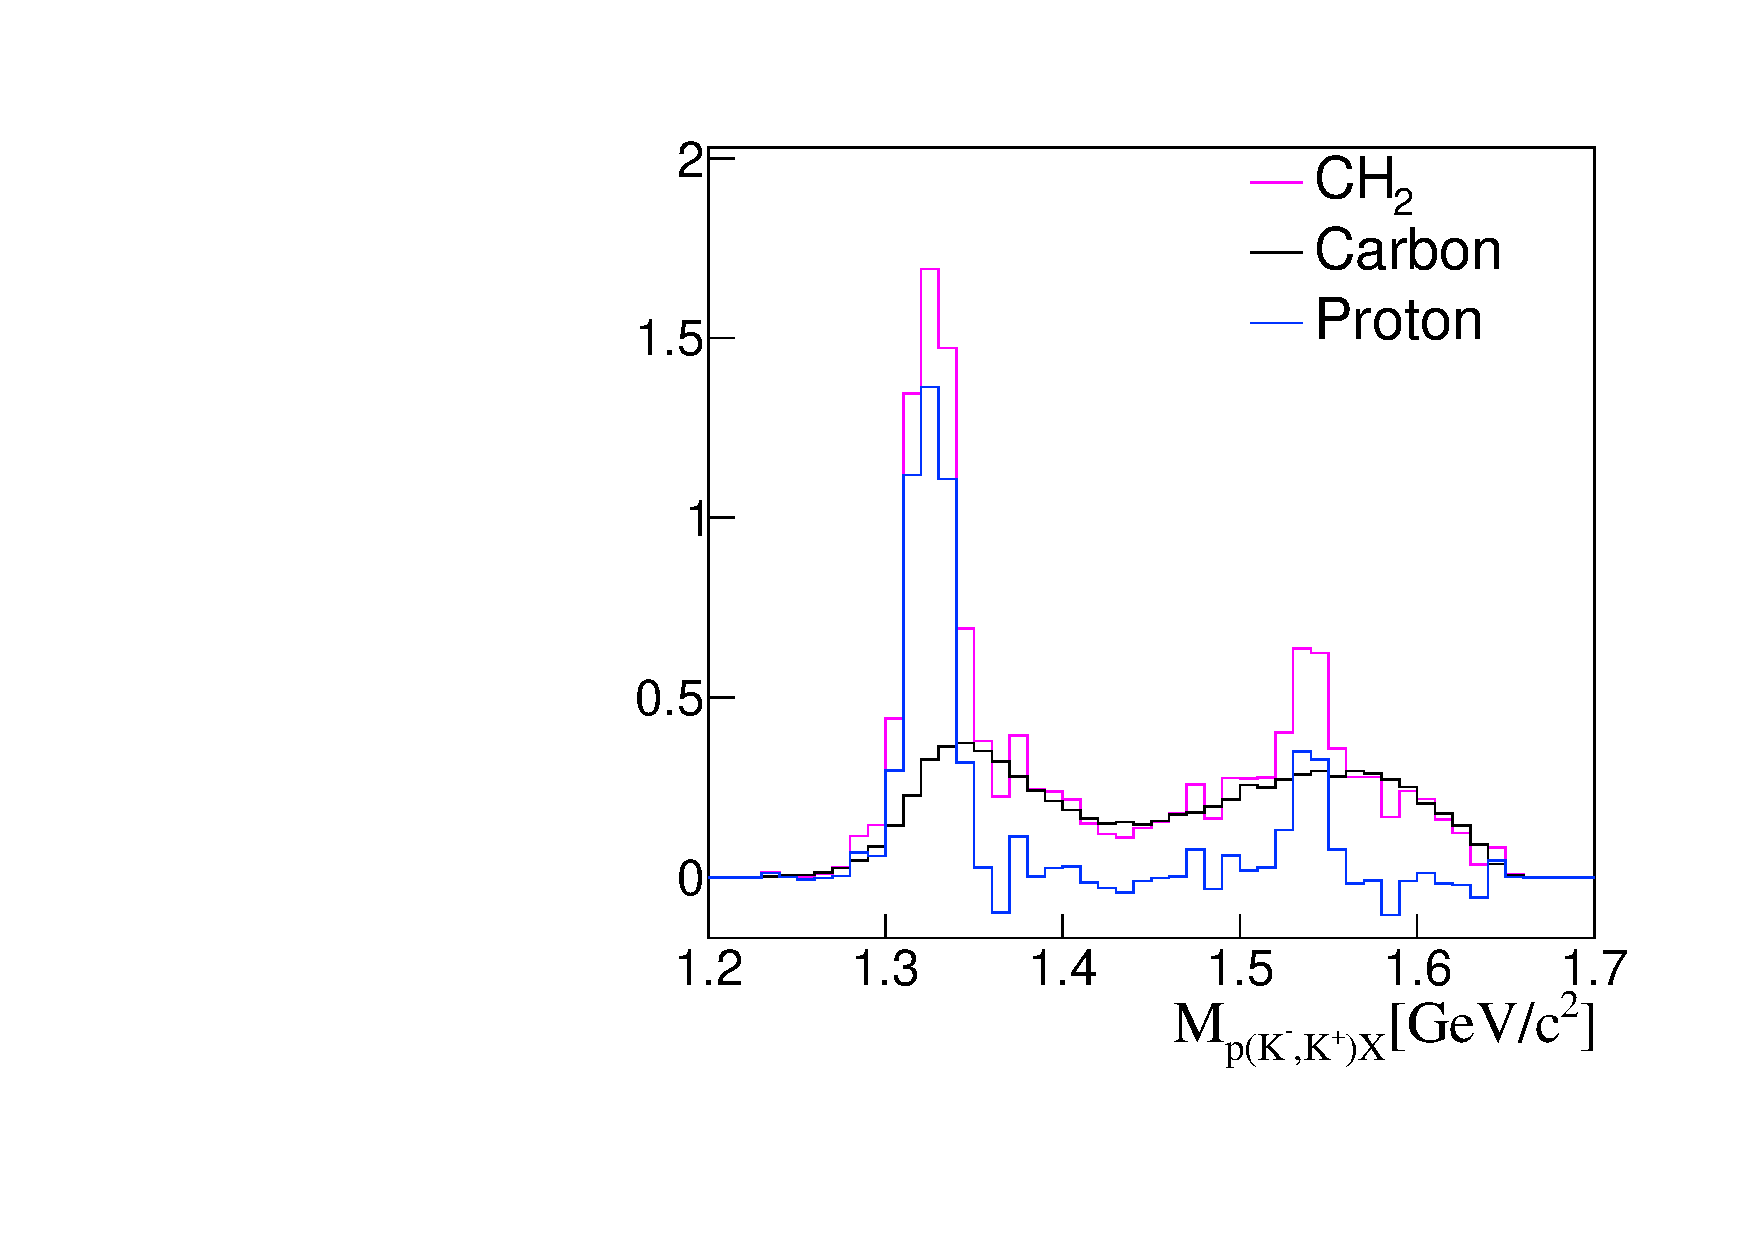
\includegraphics[width = .85\textwidth]{ProtonMMCorr}}
			\put(75,160){\large $\Xi^-$}	
			\put(125,120){\large $\Xi^{*-}$}	
			\put(60,80){\rotatebox{15}{\Huge\textcolor{tubsgray20}{Preliminary}}}
		\end{picture}
	\end{figure}
	}
\end{frame}
\begin{frame}{HypTPC}
	\tcl{8}{8}{
				\begin{picture}(200,200)
			\put(20,-10){
				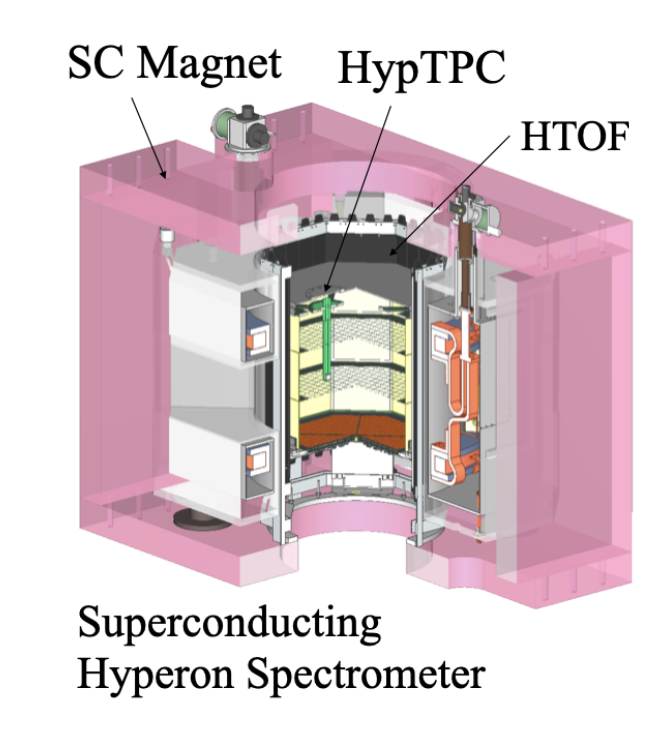
\includegraphics[width=.87\textwidth]{HypTPC}		
			}
		\end{picture}		
	}{
		\begin{picture}(200,200)
			\put(0,00){
				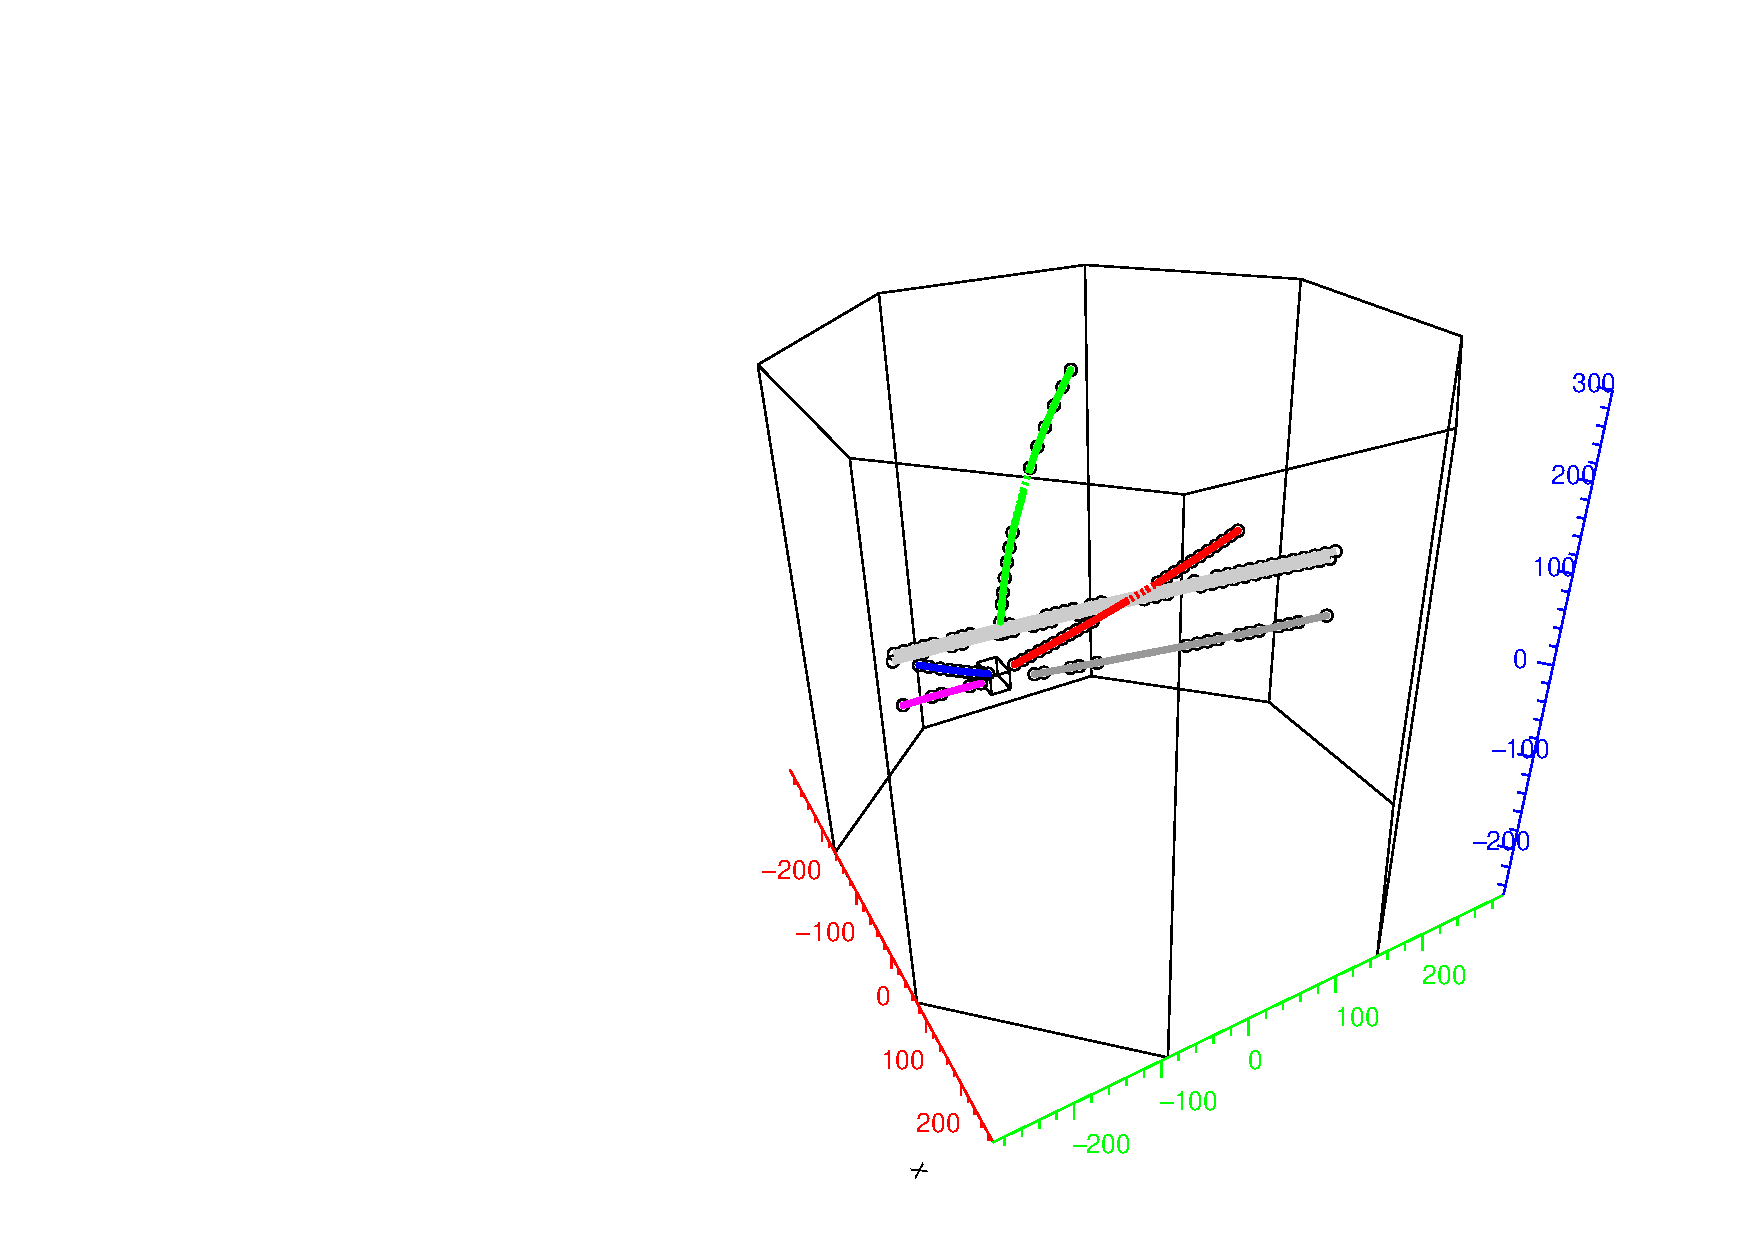
\includegraphics[width=.9\textwidth]{Run5641_Evt61424_adjusted_3D}
				\put(-150,80){\textcolor{Magenta}{\Large $K^-$}}
				\put(-90,90){\textcolor{gray}{\Large $K^+$}}
				\put(-160,110){\textcolor{Blue}{\Large $\pi_{\Xi}^-$}}
				\put(-120,150){\textcolor{Green}{\Large $\pi_{\Lambda}^-$}}
				\put(-90,125){\textcolor{Red}{\Large $p$}}
			}
		\end{picture}
		\begin{figure}
\end{figure}
	}
\end{frame}
\begin{frame}{Gluckstern Formula}
	\begin{block}{}
		\tcl{7.5}{5}{
		\begin{figure}
			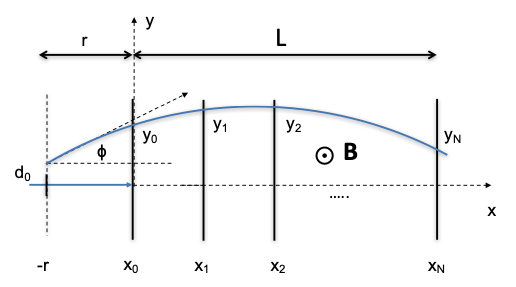
\includegraphics[width=\textwidth]{ParaLen}
		\end{figure}
		\scriptsize{Z. Drasal, W. Riegler, Nucl. Instrum. Methds. A, 910, 127-132 (2018)}
	}{
	\begin{align}
		&\frac{\sigma_{P_T}}{P_T} \simeq \frac{P_{T}}{0.3L^2B}\sqrt{\frac{720}{N+4}}\sigma_T\\
		&\frac{\sigma_{P_T,m.s}}{P_T} \simeq\frac{0.0136^1}{0,3\beta B L}\sqrt{\frac{d_{tot}}{X_0}}
	\end{align}
	{\scriptsize{Units in GeV/c}}
	\begin{itemize}
		\item Momentum resolution comprises geometrical term and scattering term
		\item In practice, empirical rescaling factor should be multiplied
	\end{itemize}
	\scriptsize{$^1$G.R. Lynch and O.I Dahl, Nucl. Instrum. Methods B58, 6 (1991).}
	}
	\end{block}
\end{frame}
\begin{frame}{Covariance Matrix in Helix Track}
	\begin{block}{}
		\tcl{3}{6}{
			\vspace{-7 mm}
			\begin{figure}
				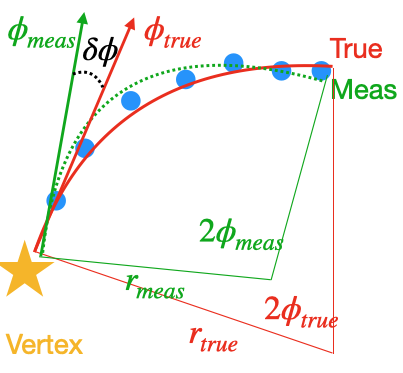
\includegraphics[width=4 cm]{PT_Phi}
			\end{figure}
		}
		{
			\begin{itemize}
				\item Variance in momentum modifies the curvature of the helix $\to$ direction at the vertex changes.
				\item 'Position' of the helix is defined from the TPC hits. $\to $ Center-of-gravity should be fixed.
			\end{itemize} 
		}
		Denote the tangent angle at the center be $\phi_0$ and path length to the vertex $l$.
		\begin{align}
			\phi = \phi_0 \pm \frac{l}{2r};\quad  \delta\phi = \pm\frac{l}{2r}\frac{\delta r}{r}= \pm\frac{l}{r}\frac{\delta p_T}{p_T}
		\end{align}
		\begin{align}
			\sigma_{\phi}^2 = \langle\delta\phi\delta\phi\rangle=\frac{l^2}{r^2p_{T}^2}\sigma^2_{p_T};\quad \textrm{Cov}(\phi,p_T)= \langle\delta\phi\delta p_T \rangle = \pm \frac{l}{rp_T}\sigma_{p_T}^2
		\end{align}
	\end{block}
\end{frame}
\begin{frame}{Covariance Matrix in Helix Track}
	\begin{block}{}
		\tcl{4}{7}{
			\vspace{-7 mm}
			\begin{figure}
				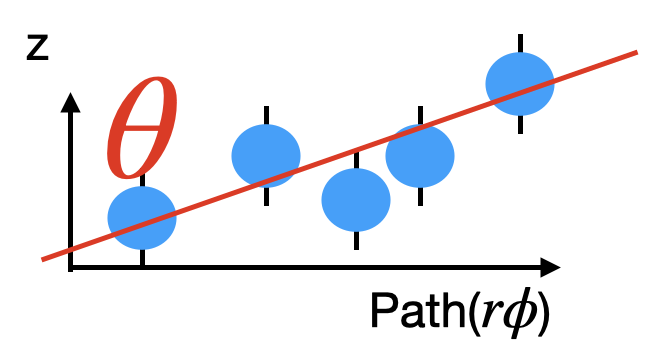
\includegraphics[width=5 cm]{Res_Th}
			\end{figure}
		}
		{
			\begin{align}
				h(t): \{r\cos(\phi ) - c_x , r\sin\phi - c_y,  dz*r\phi - z_0\}\label{EqHelix}
			\end{align}
			\begin{itemize}
				\item The 'pitch' parameter, dz, is the slope along the circular trajectory
			\end{itemize}
		}
		\vspace{3 mm}
		$\theta = \frac{\pi}{2}-\arctan(dz)$, we estimate the variance of $\theta$ based on the fitting error of dz. The error is estimated from the slope error of a linear fit: 
		\begin{align*}
			\sigma_{dz}^2 =\frac{\sum\delta_z^2/(n-2) }{\sum(x-\bar x)^2} \simeq \frac{n \sigma_z^2/(n-2)}{n L^2/12};\quad \sigma_\theta = \pdf{dz}{\theta}\sigma_{dz}=\frac{1}{1+dz^2}\sigma_{dz}.
		\end{align*}
		Note that, the momentum $p_z=p_T dz$ would also have some covariance with $\theta$,
		\begin{align*}
			\langle \delta p\delta \theta\rangle = dz\langle  \ctz{\delta p_T  \delta \theta}\rangle+	p_T\langle \delta dz \delta \theta\rangle =\frac{p_T}{1+dz^2}\sigma_{dz}^2.
		\end{align*}
	\end{block}
\end{frame}
\begin{frame}{$\phi$ Restoration from Diagonal Component}
\tcl{8}{8}{
	\begin{figure}
		\begin{picture}(200,150)
			\put(-10,0){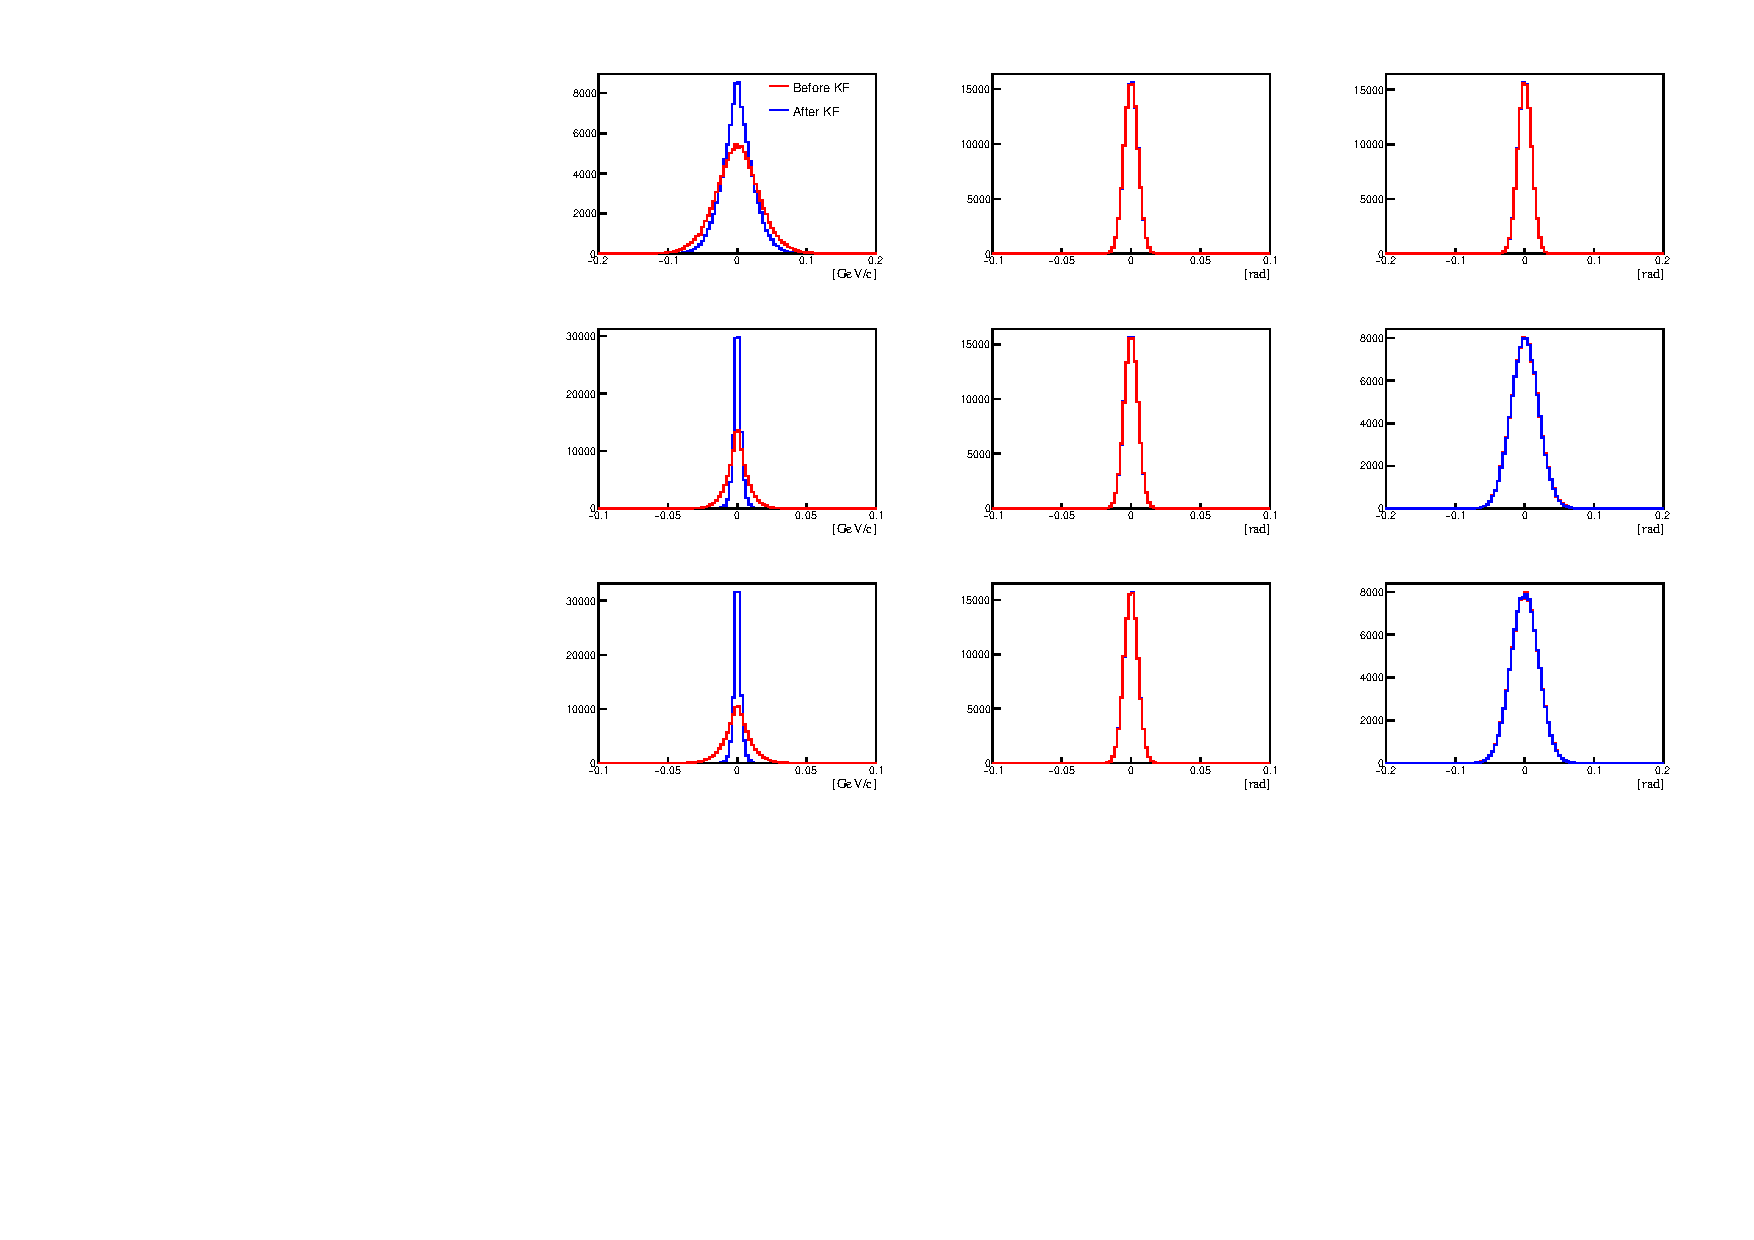
\includegraphics[width=.95\textwidth]{Xi_cKF1}}
			\put(30,40){\rotatebox{15}{\Huge\textcolor{tubsgray20}{ToySimulation}}}
		\end{picture}		
	\end{figure}
}{
	\begin{figure}
		\begin{picture}(200,150)
			\put(-10,0){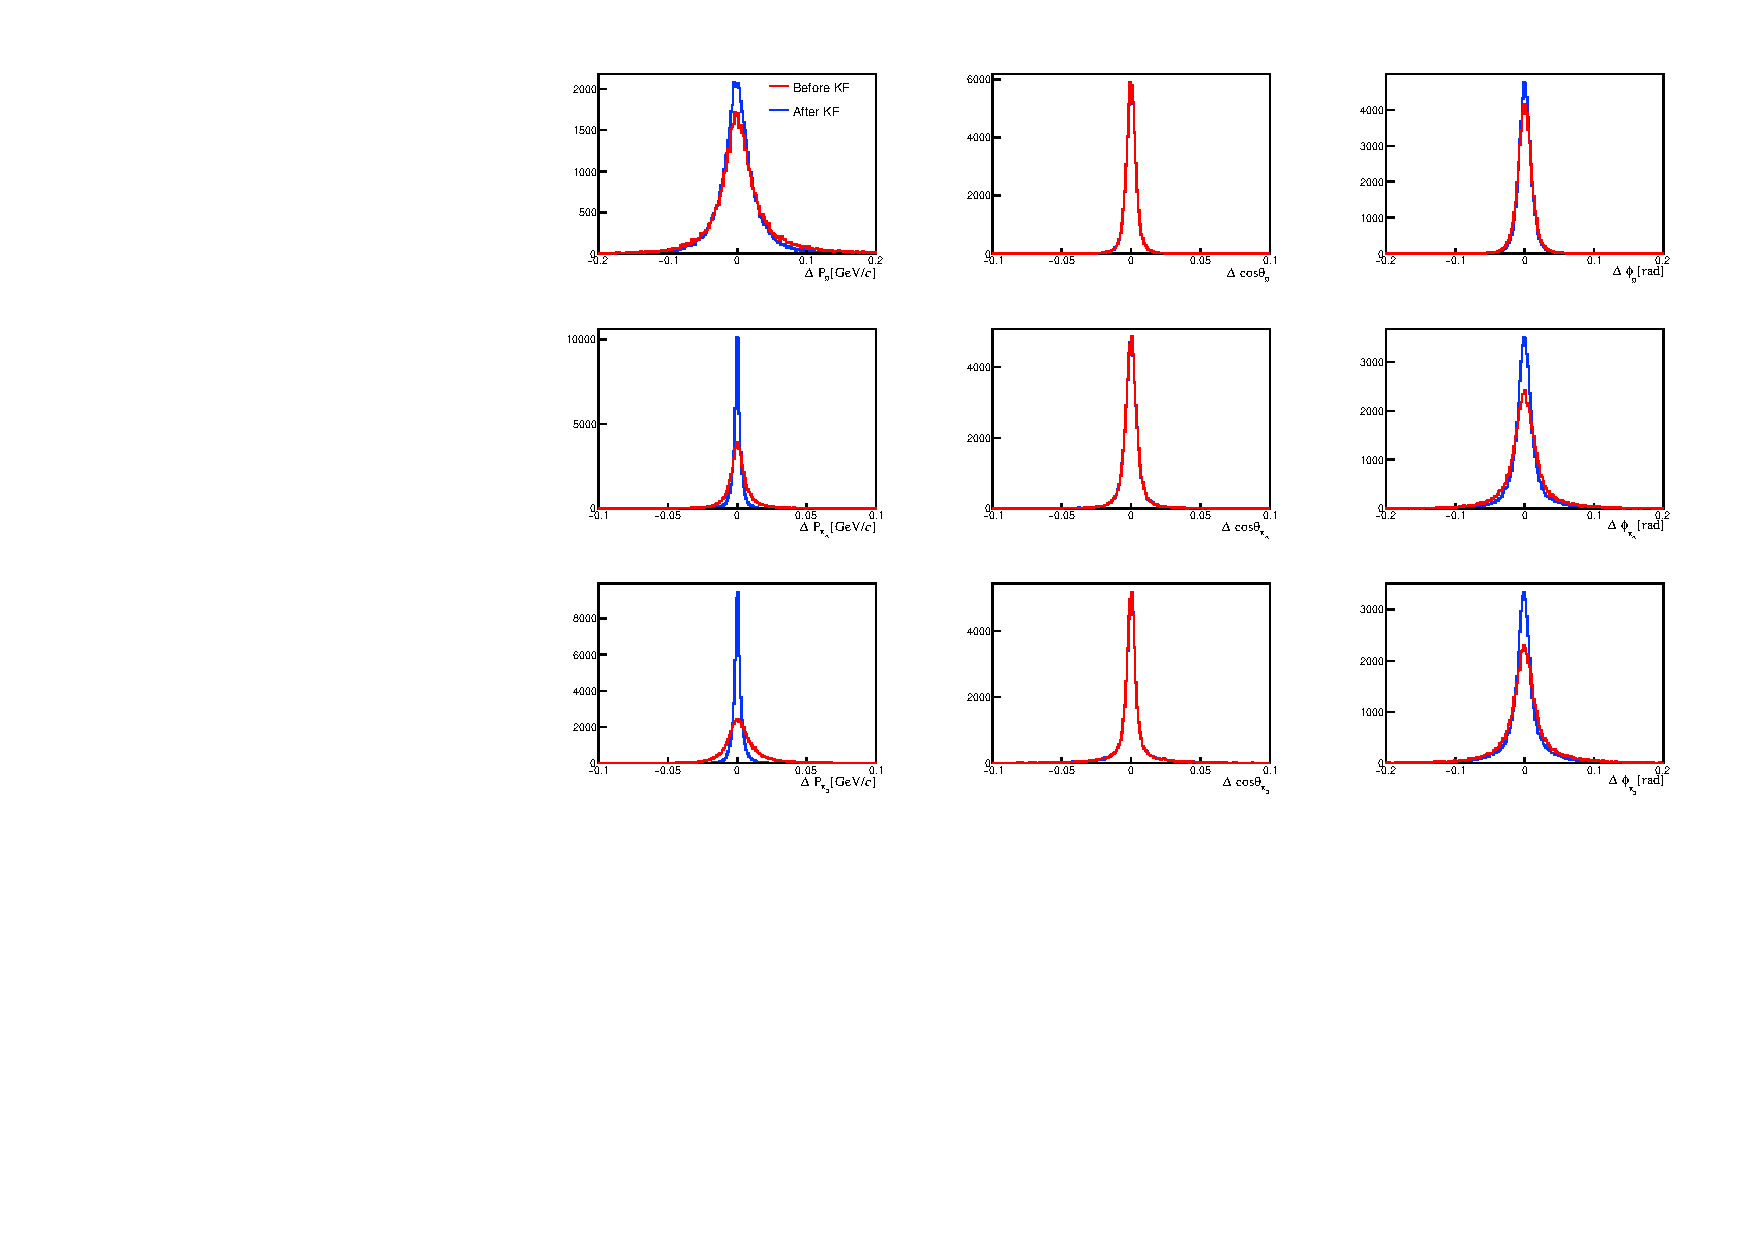
\includegraphics[width=.95\textwidth]{KF_DaughterStatus}}
			\put(30,40){\rotatebox{15}{\Huge\textcolor{tubsgray20}{E42 Geant4}}}
		\end{picture}		
	\end{figure}
}
\end{frame}
\begin{frame}{Invariant Mass Bending from Momentum Bias}
	\tcl{8}{8}{
		\begin{figure}
			\begin{picture}(200,150)
				\put(-10,-30){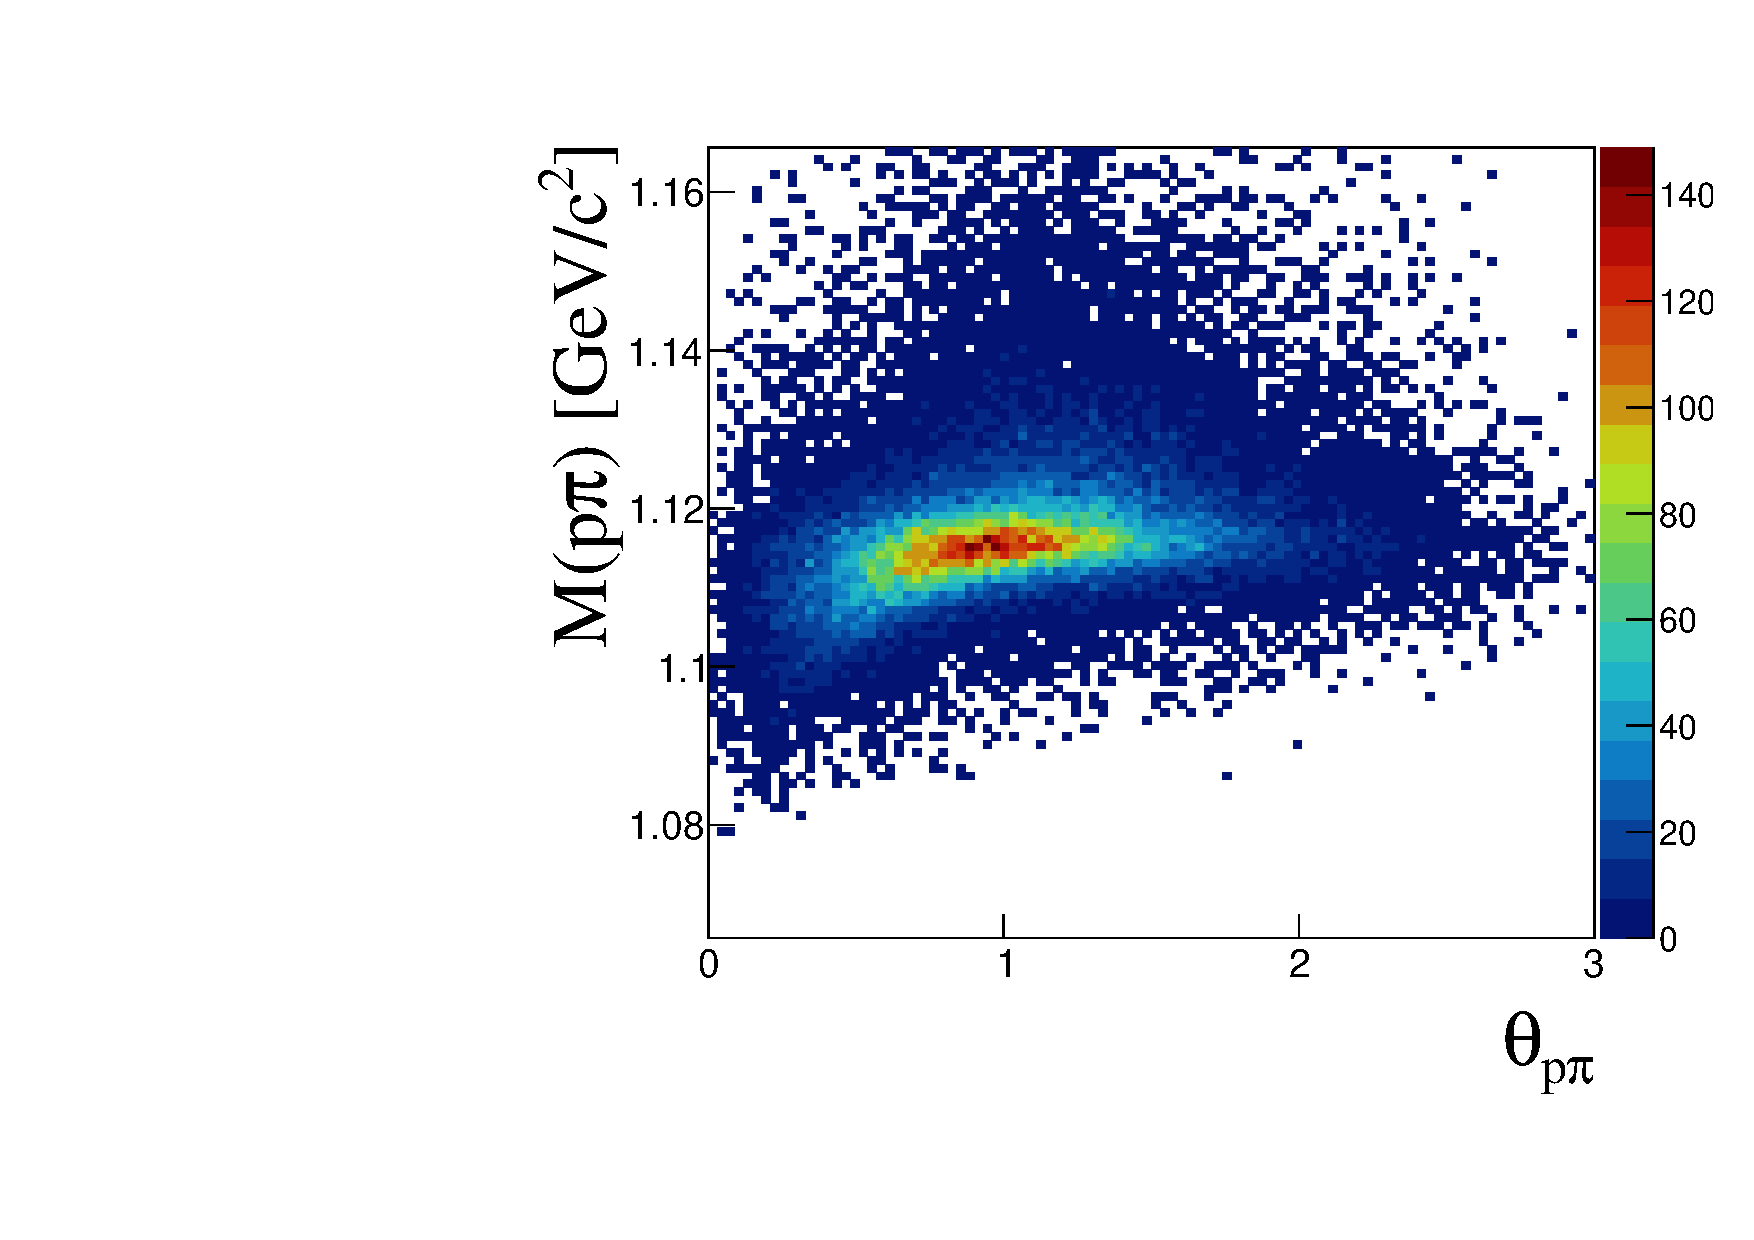
\includegraphics[width=.95\textwidth]{hLambdaOpening_Mass_CutStandard}}
				\put(30,50){\rotatebox{15}{\Huge\textcolor{tubsgray20}{Preliminary}}}
			\end{picture}		
		\end{figure}
	}{
			\begin{figure}
		\begin{picture}(200,150)
			\put(-10,-30){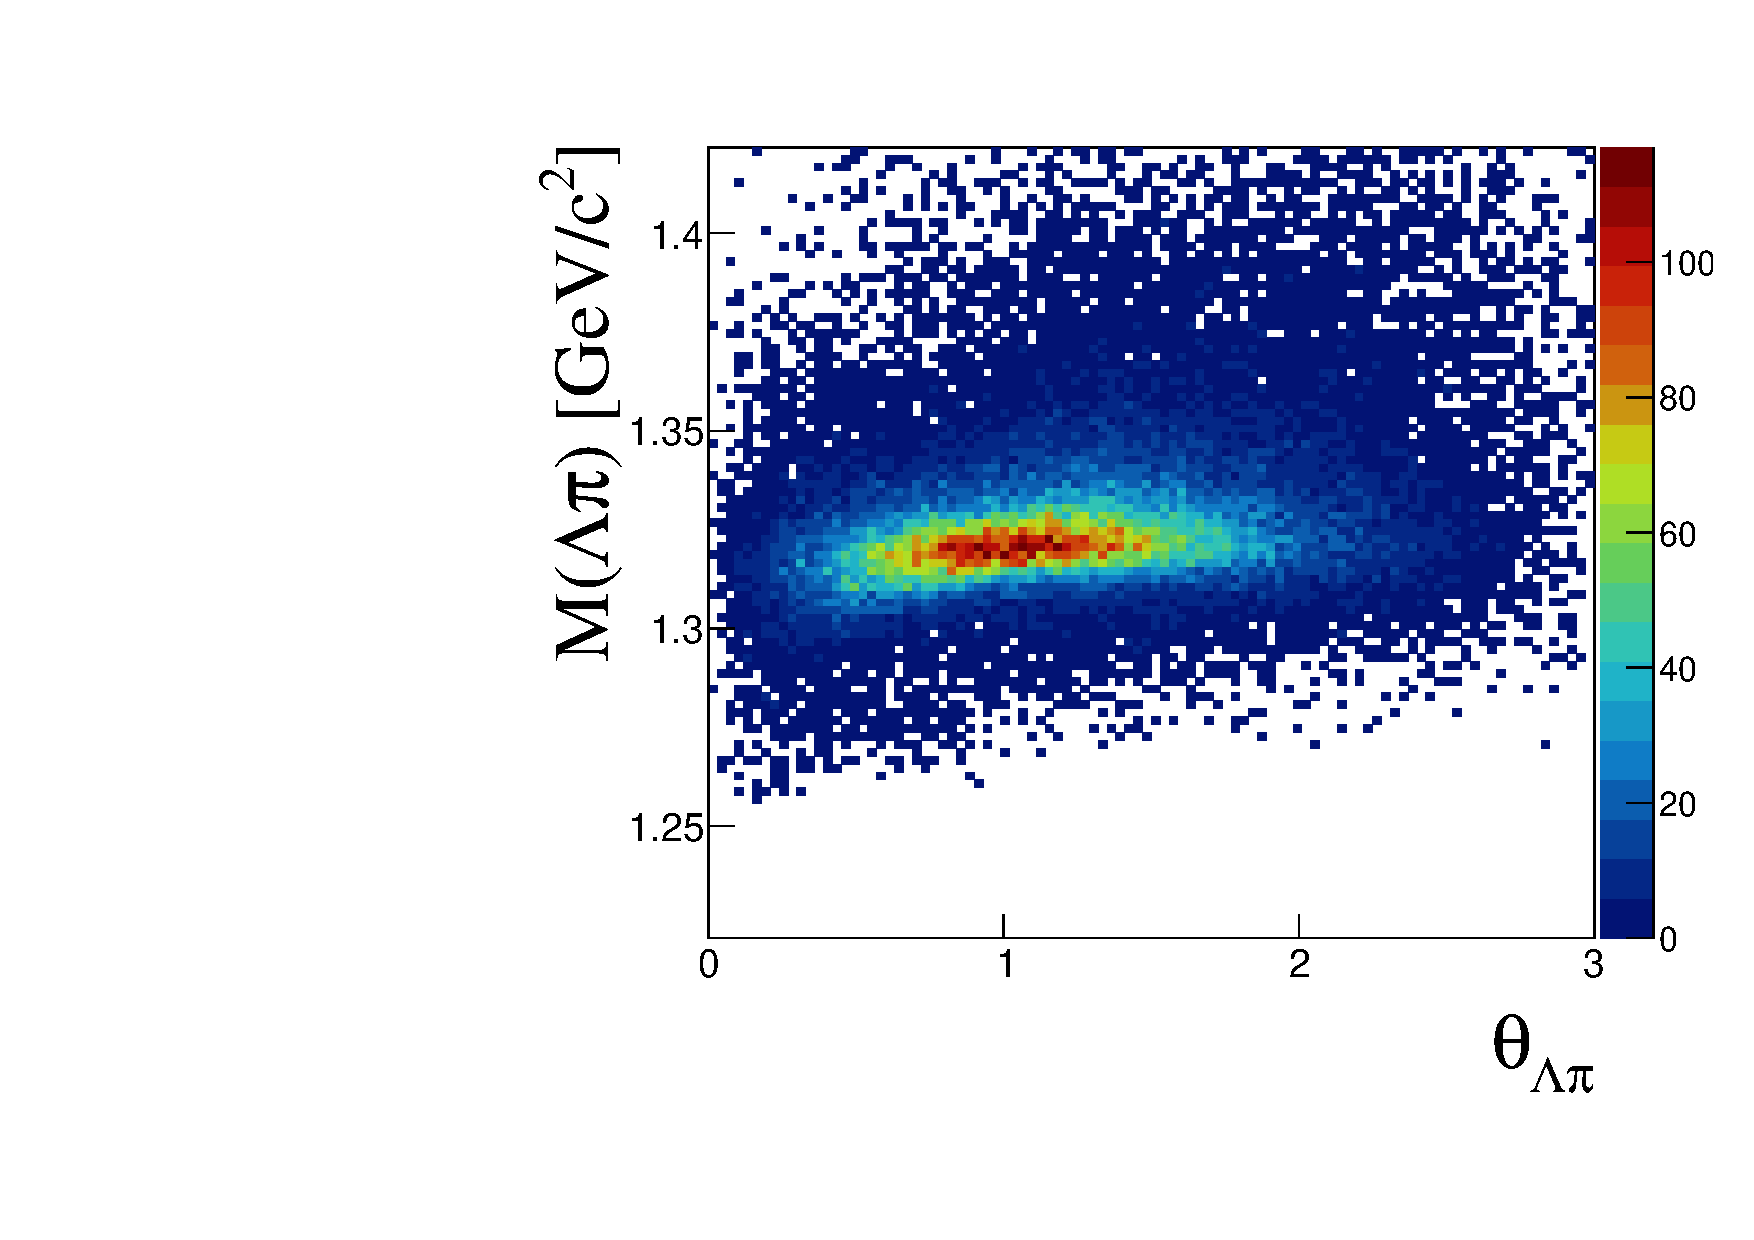
\includegraphics[width=.95\textwidth]{hXiOpening_Mass_CutStandard}}
			\put(30,50){\rotatebox{15}{\Huge\textcolor{tubsgray20}{Preliminary}}}
		\end{picture}		
	\end{figure}
	}
\end{frame}
\begin{frame}{Off-center Pull Distribution}
\begin{figure}
	\begin{picture}(200,150)
		\put(0,0){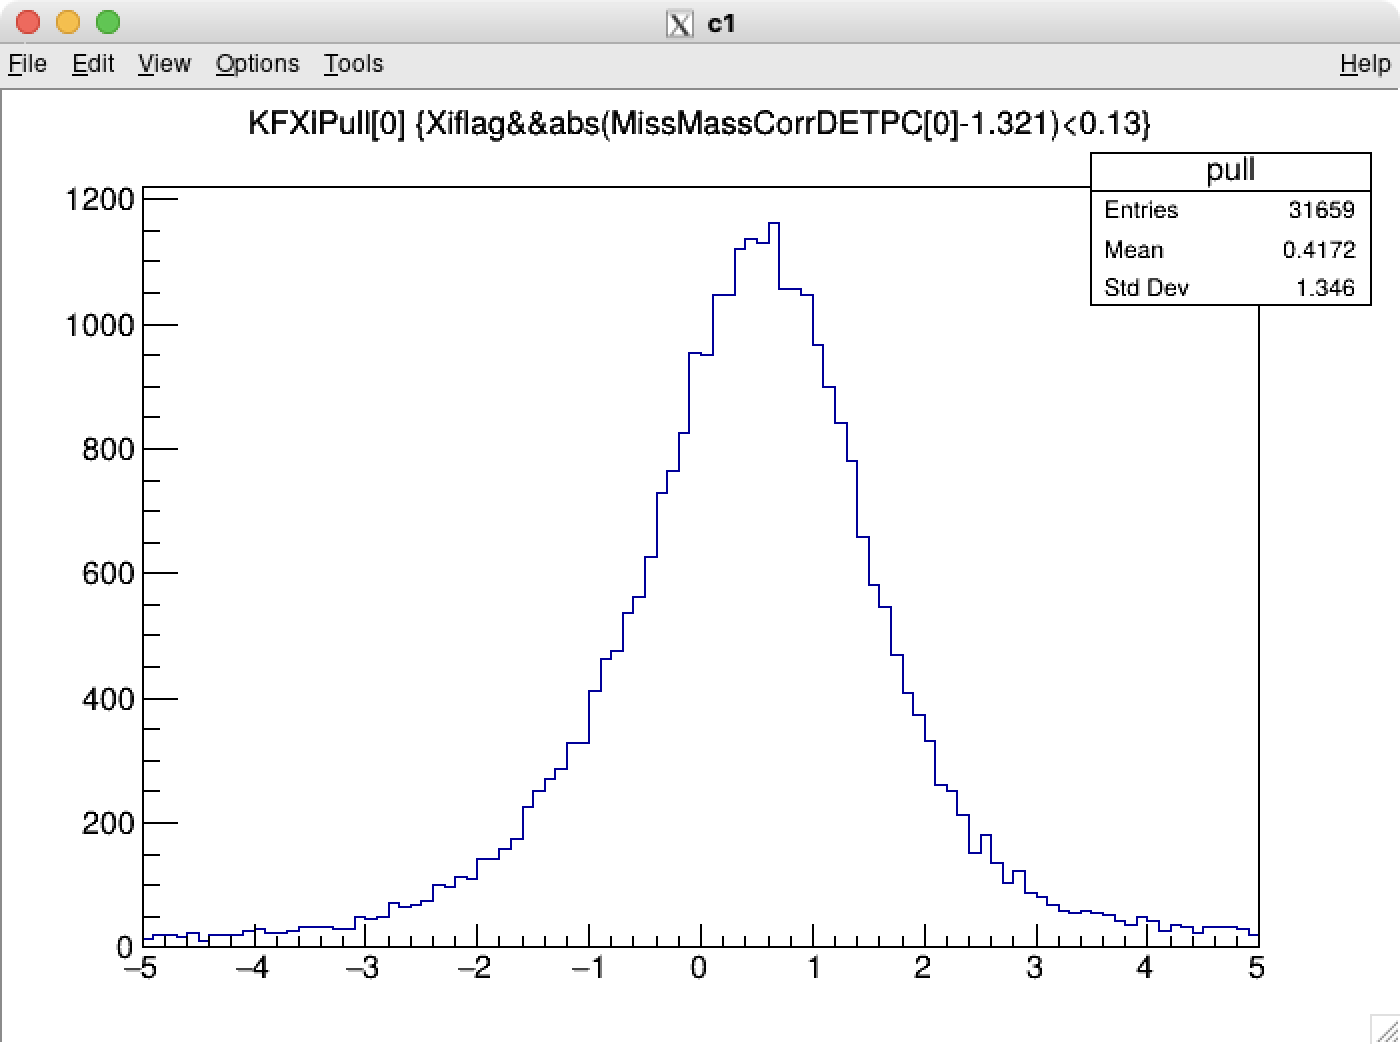
\includegraphics[width=.95\textwidth]{Xi_Pull_Before}}
		\put(30,50){\rotatebox{15}{\Huge\textcolor{tubsgray20}{Preliminary}}}
	\end{picture}		
\end{figure}
\end{frame}
\begin{frame}{Position Residual?}
	\tcl{8}{8}
{
	\begin{figure}
		\begin{picture}(200,150)
			\put(-10,20){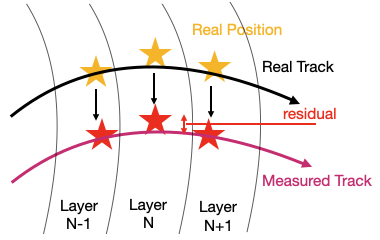
\includegraphics[width=.95\textwidth]{DistortionCartoon}}
		\end{picture}		
	\end{figure}
}
	{
	\begin{figure}
		\begin{picture}(200,150)
			\put(-10,30){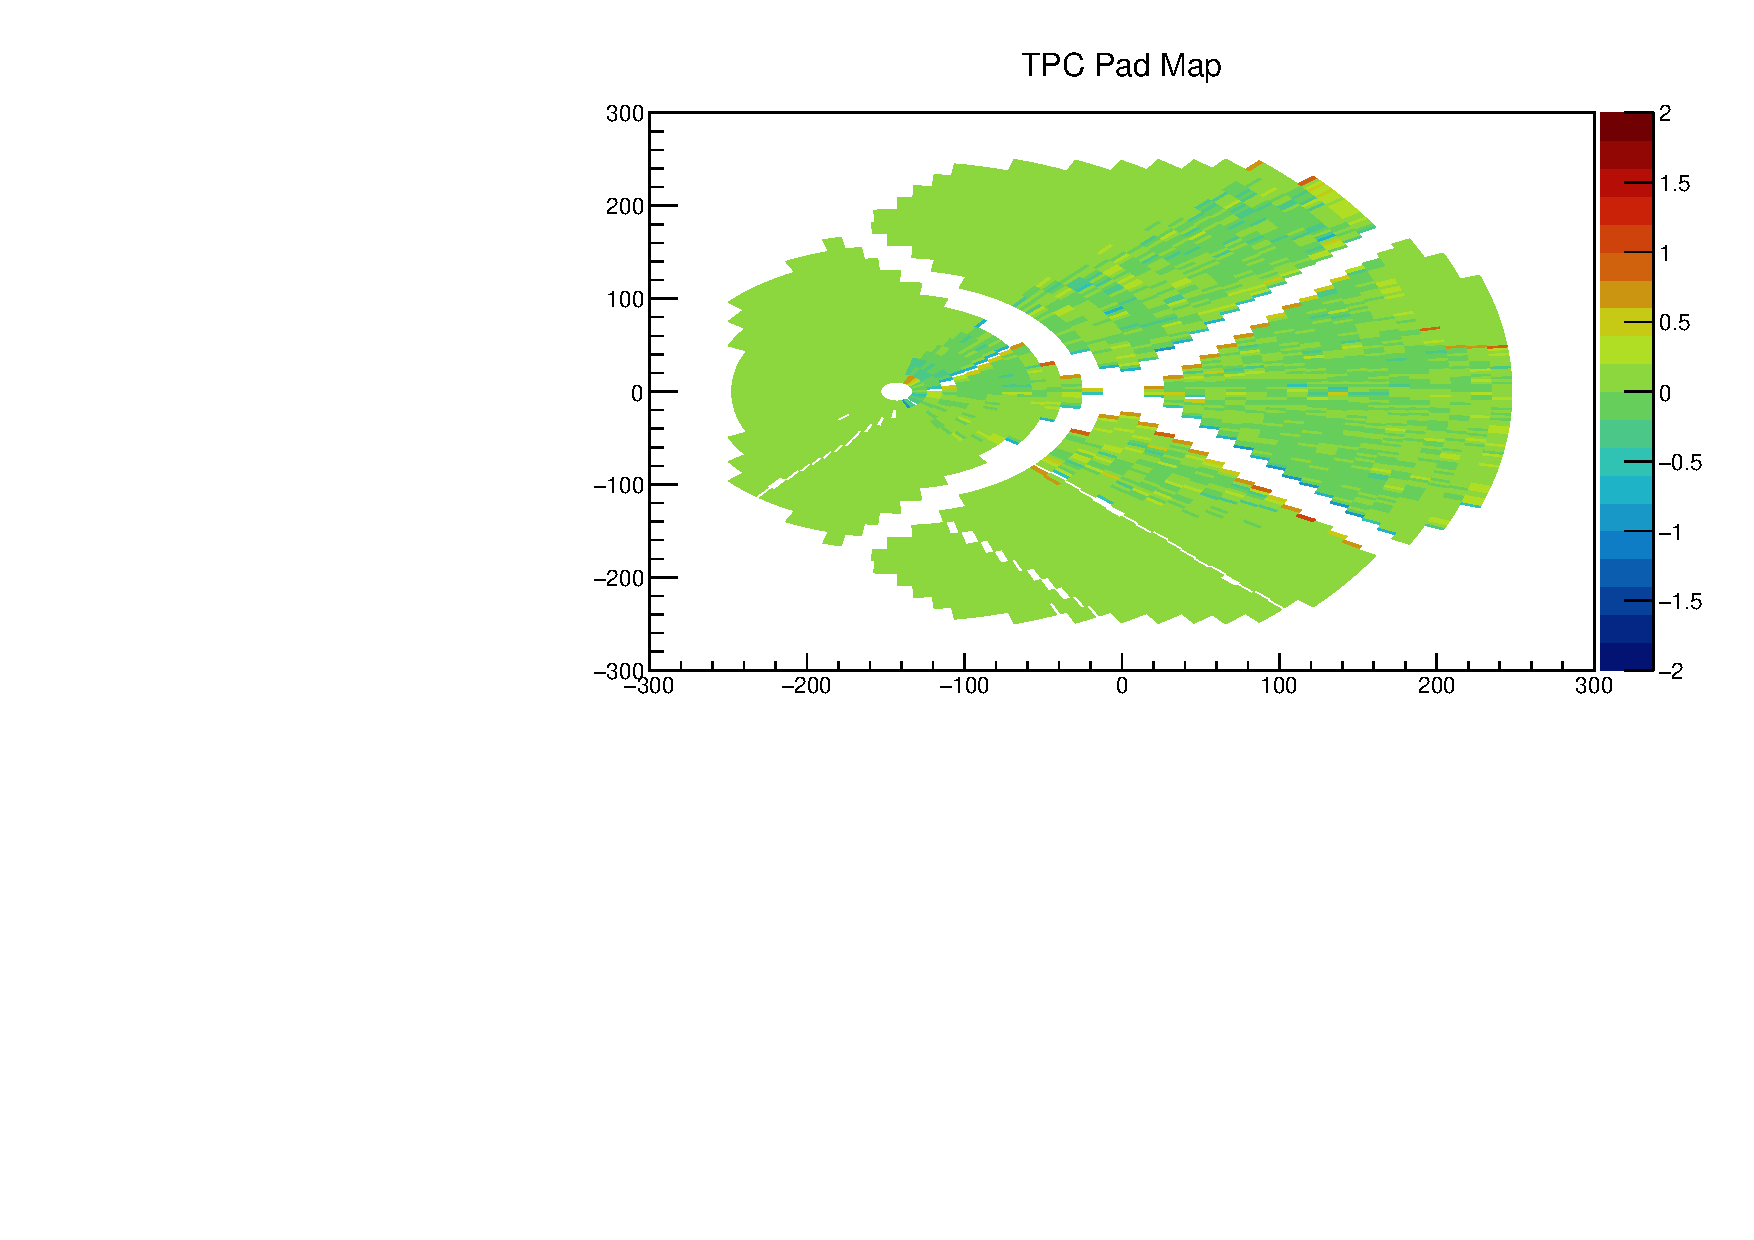
\includegraphics[width=.95\textwidth]{Before/c_pad_r}}
			\put(30,80){\rotatebox{15}{\Huge\textcolor{tubsgray20}{Preliminary}}}
		\end{picture}		
	\end{figure}
}
\begin{block}{}
	\begin{itemize}
		\item Local, but simultaneous shift cannot be detected from position residual measurement.
		\item External reference for track should be provided to estimate 'true' trajectory
	\end{itemize}
\end{block}
\end{frame}
\begin{frame}{Position Residual from KF Track}
	\tcl{8}{8}
{
	\begin{figure}
		\begin{picture}(200,150)
			\put(-10,20){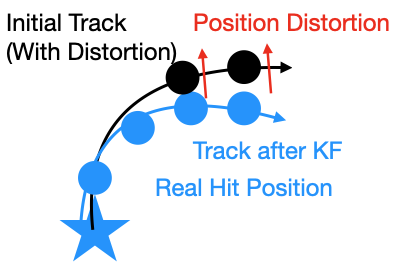
\includegraphics[width=.95\textwidth]{FitCartoon}}
		\end{picture}		
	\end{figure}
}
{
	\begin{figure}
		\begin{picture}(200,150)
			\put(-10,30){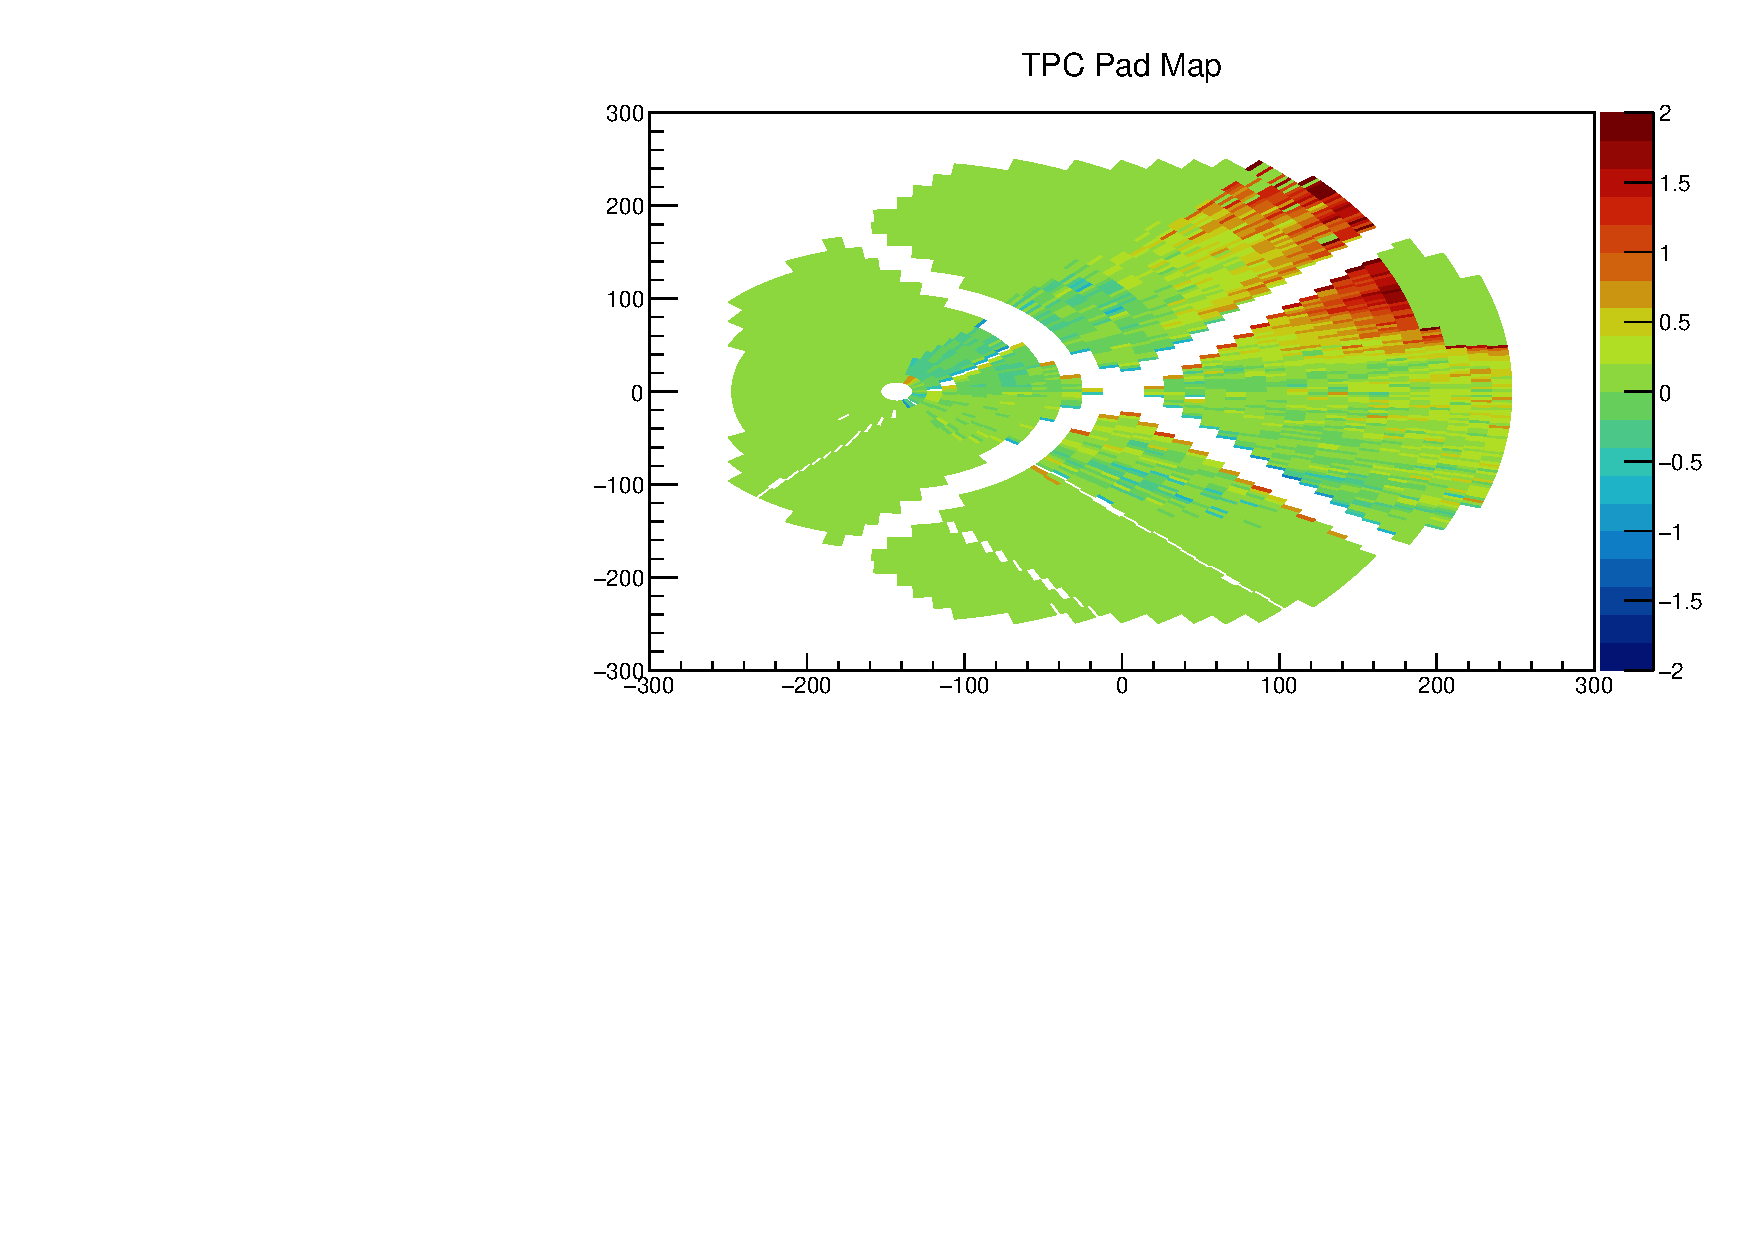
\includegraphics[width=.95\textwidth]{Before/c_pad_KF_r}}
			\put(30,80){\rotatebox{15}{\Huge\textcolor{tubsgray20}{Preliminary}}}
		\end{picture}		
	\end{figure}
}
\begin{block}{}
	\begin{itemize}
		\item From Kinematic fit, 'true' momentum, hence trajectory is estimated
	\end{itemize}
\end{block}
\end{frame}
\begin{frame}{$\Lambda$ After Position Correction}
	\tcl{8}{8}{
	\begin{figure}
		\begin{picture}(200,150)
			\put(-10,-30){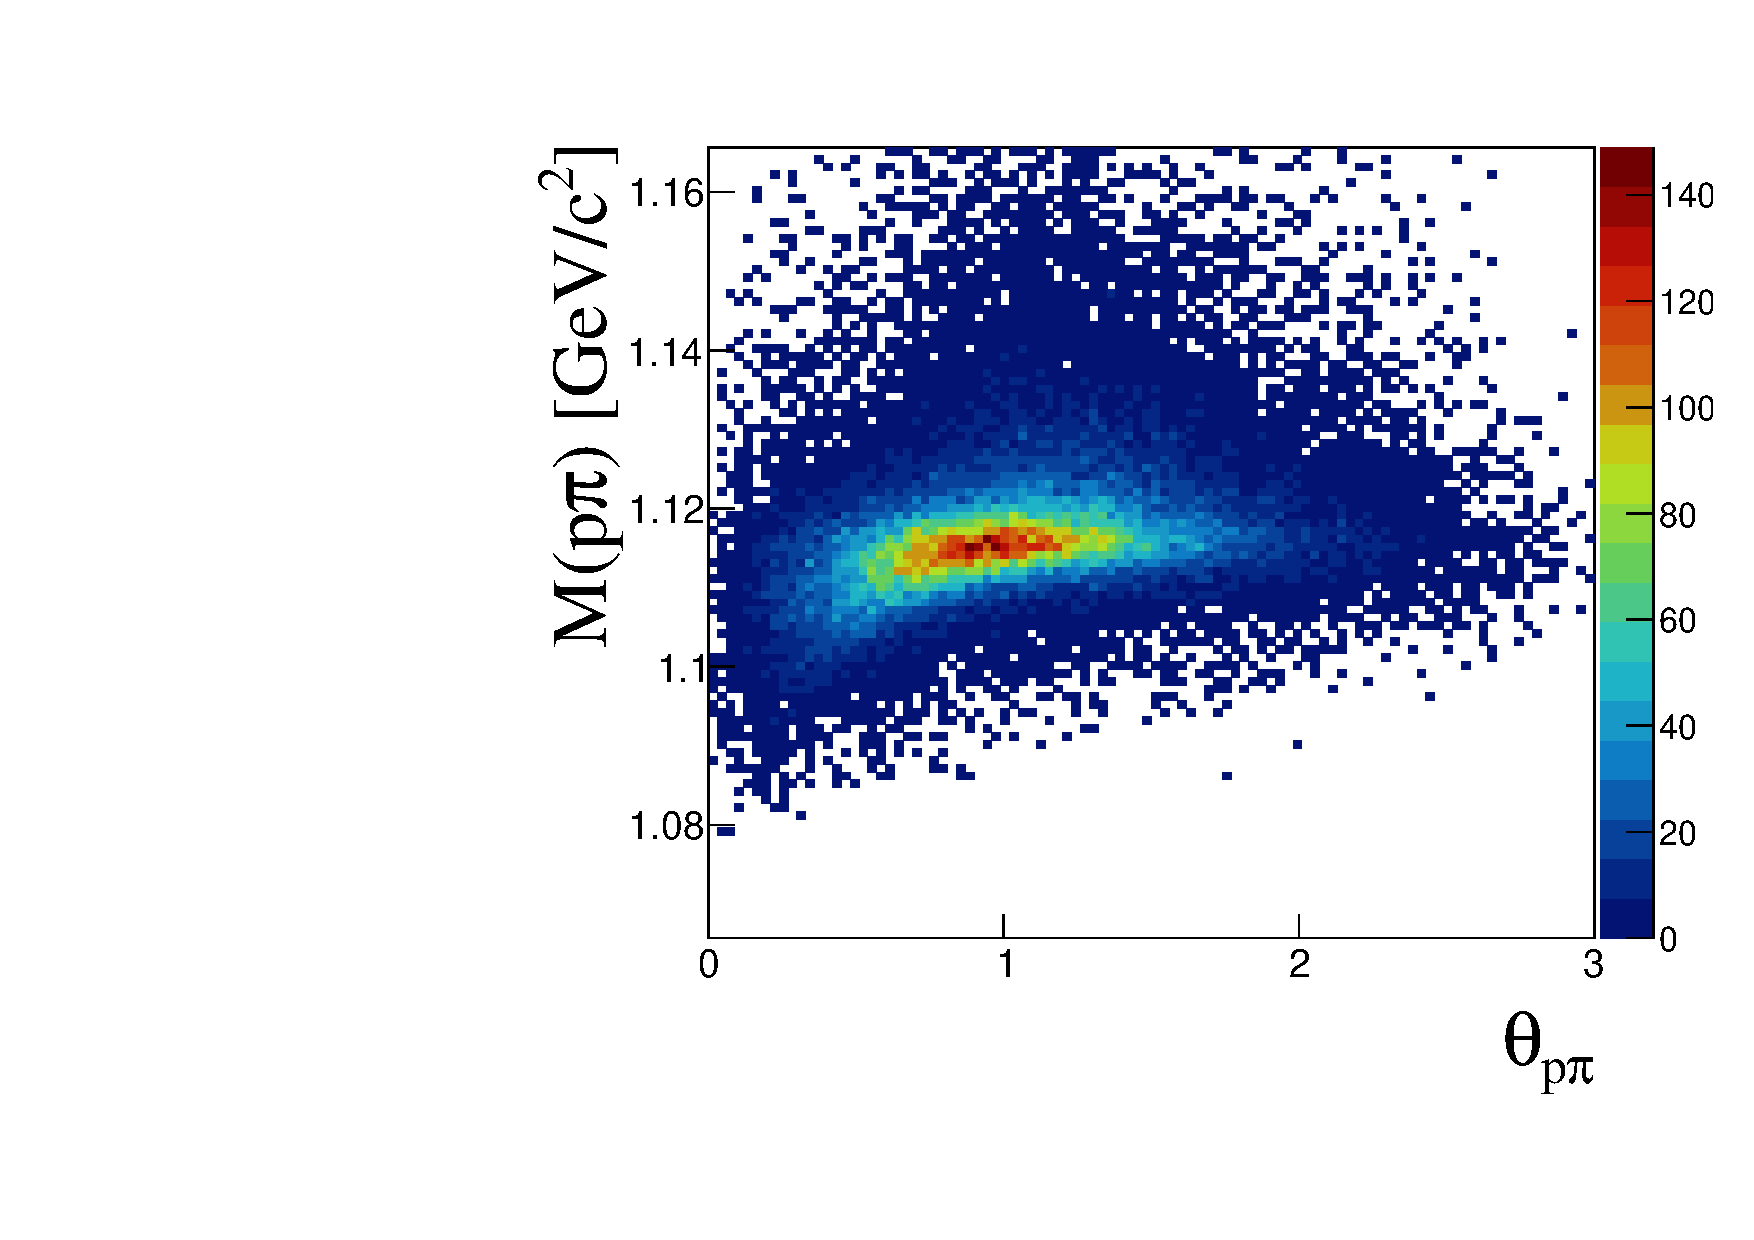
\includegraphics[width=.95\textwidth]{hLambdaOpening_Mass_CutStandard}}
			\put(30,50){\rotatebox{15}{\Huge\textcolor{tubsgray20}{Preliminary}}}
		\end{picture}		
	\end{figure}
}{
	\begin{figure}
		\begin{picture}(200,150)
			\put(-10,-30){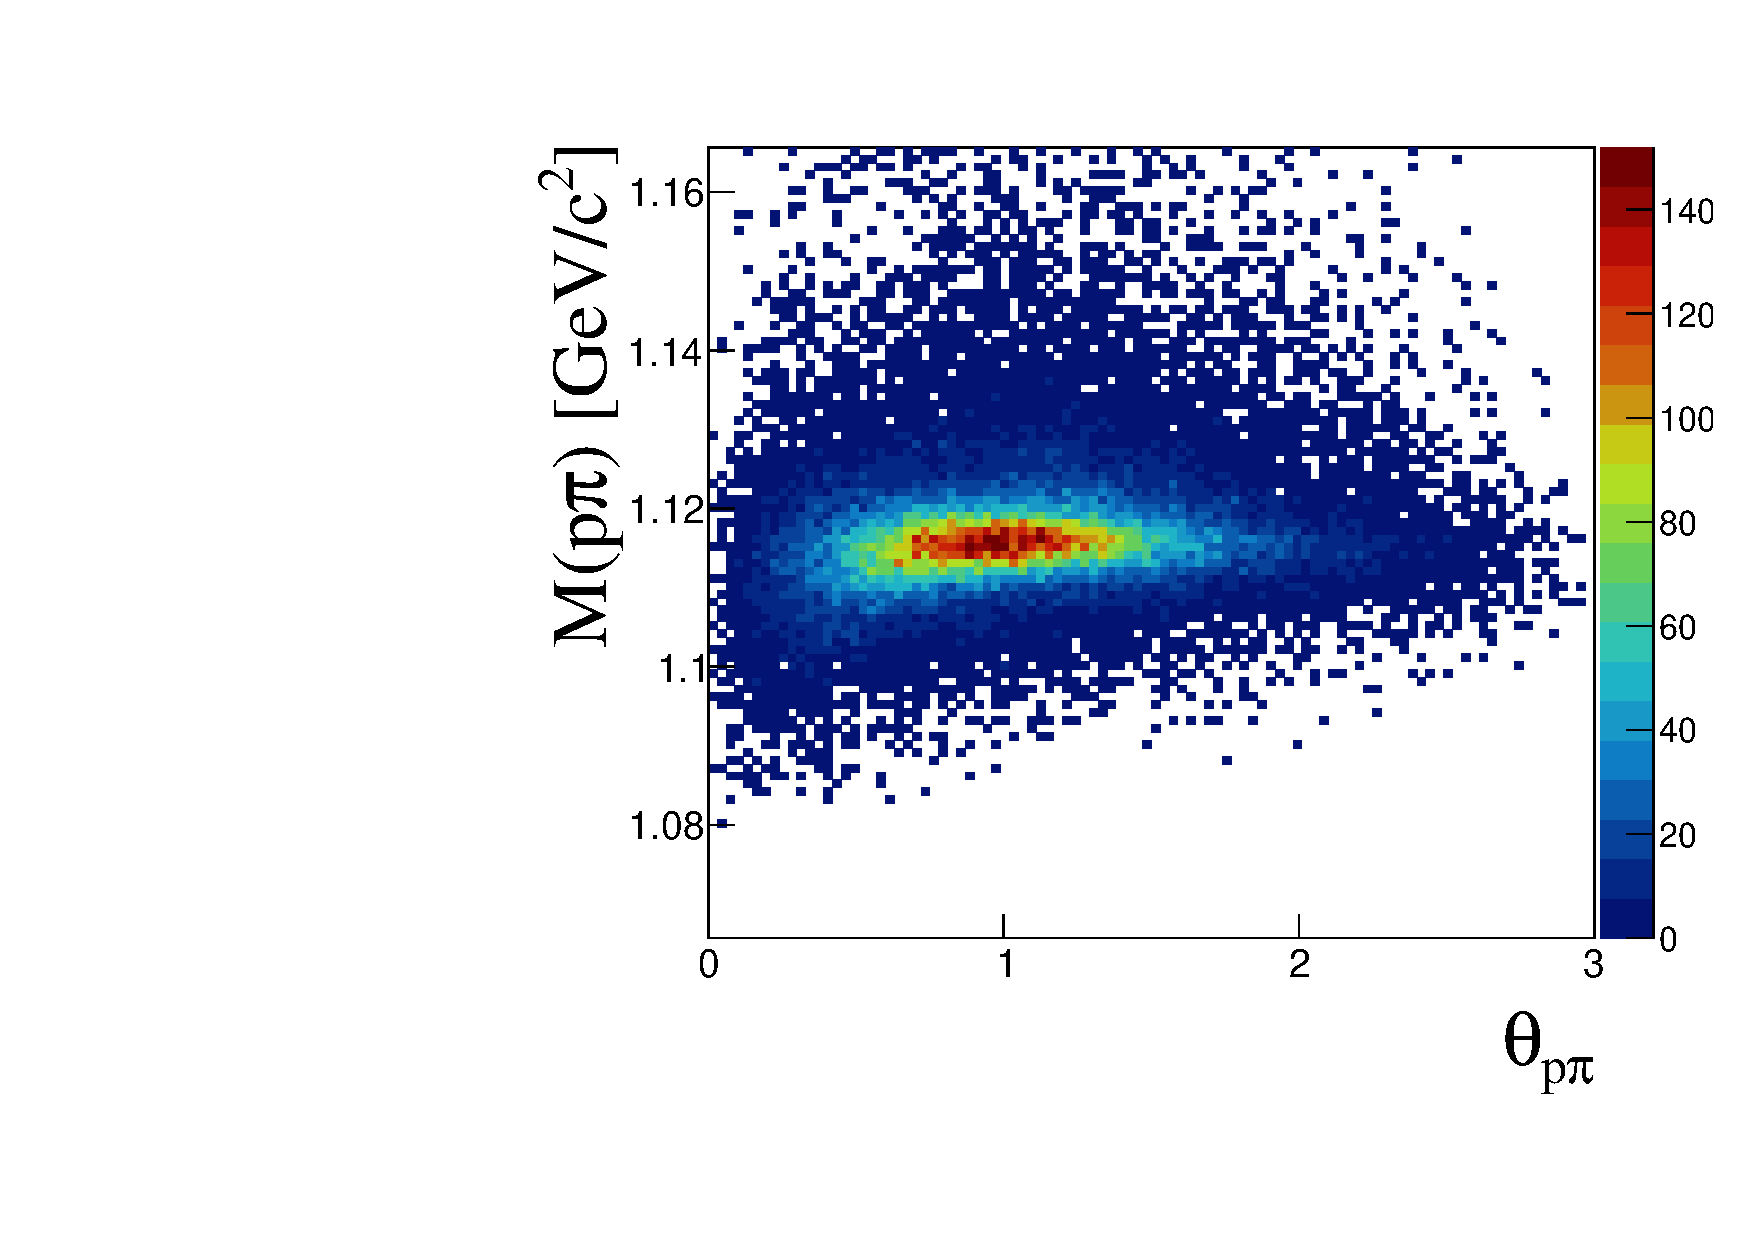
\includegraphics[width=.95\textwidth]{hLambdaOpening_Mass_CutCor}}
			\put(30,50){\rotatebox{15}{\Huge\textcolor{tubsgray20}{Preliminary}}}
		\end{picture}		
	\end{figure}
}
\end{frame}
\begin{frame}{$\Xi$ After Position Correction}
	\tcl{8}{8}{
		\begin{figure}
			\begin{picture}(200,150)
				\put(-10,-30){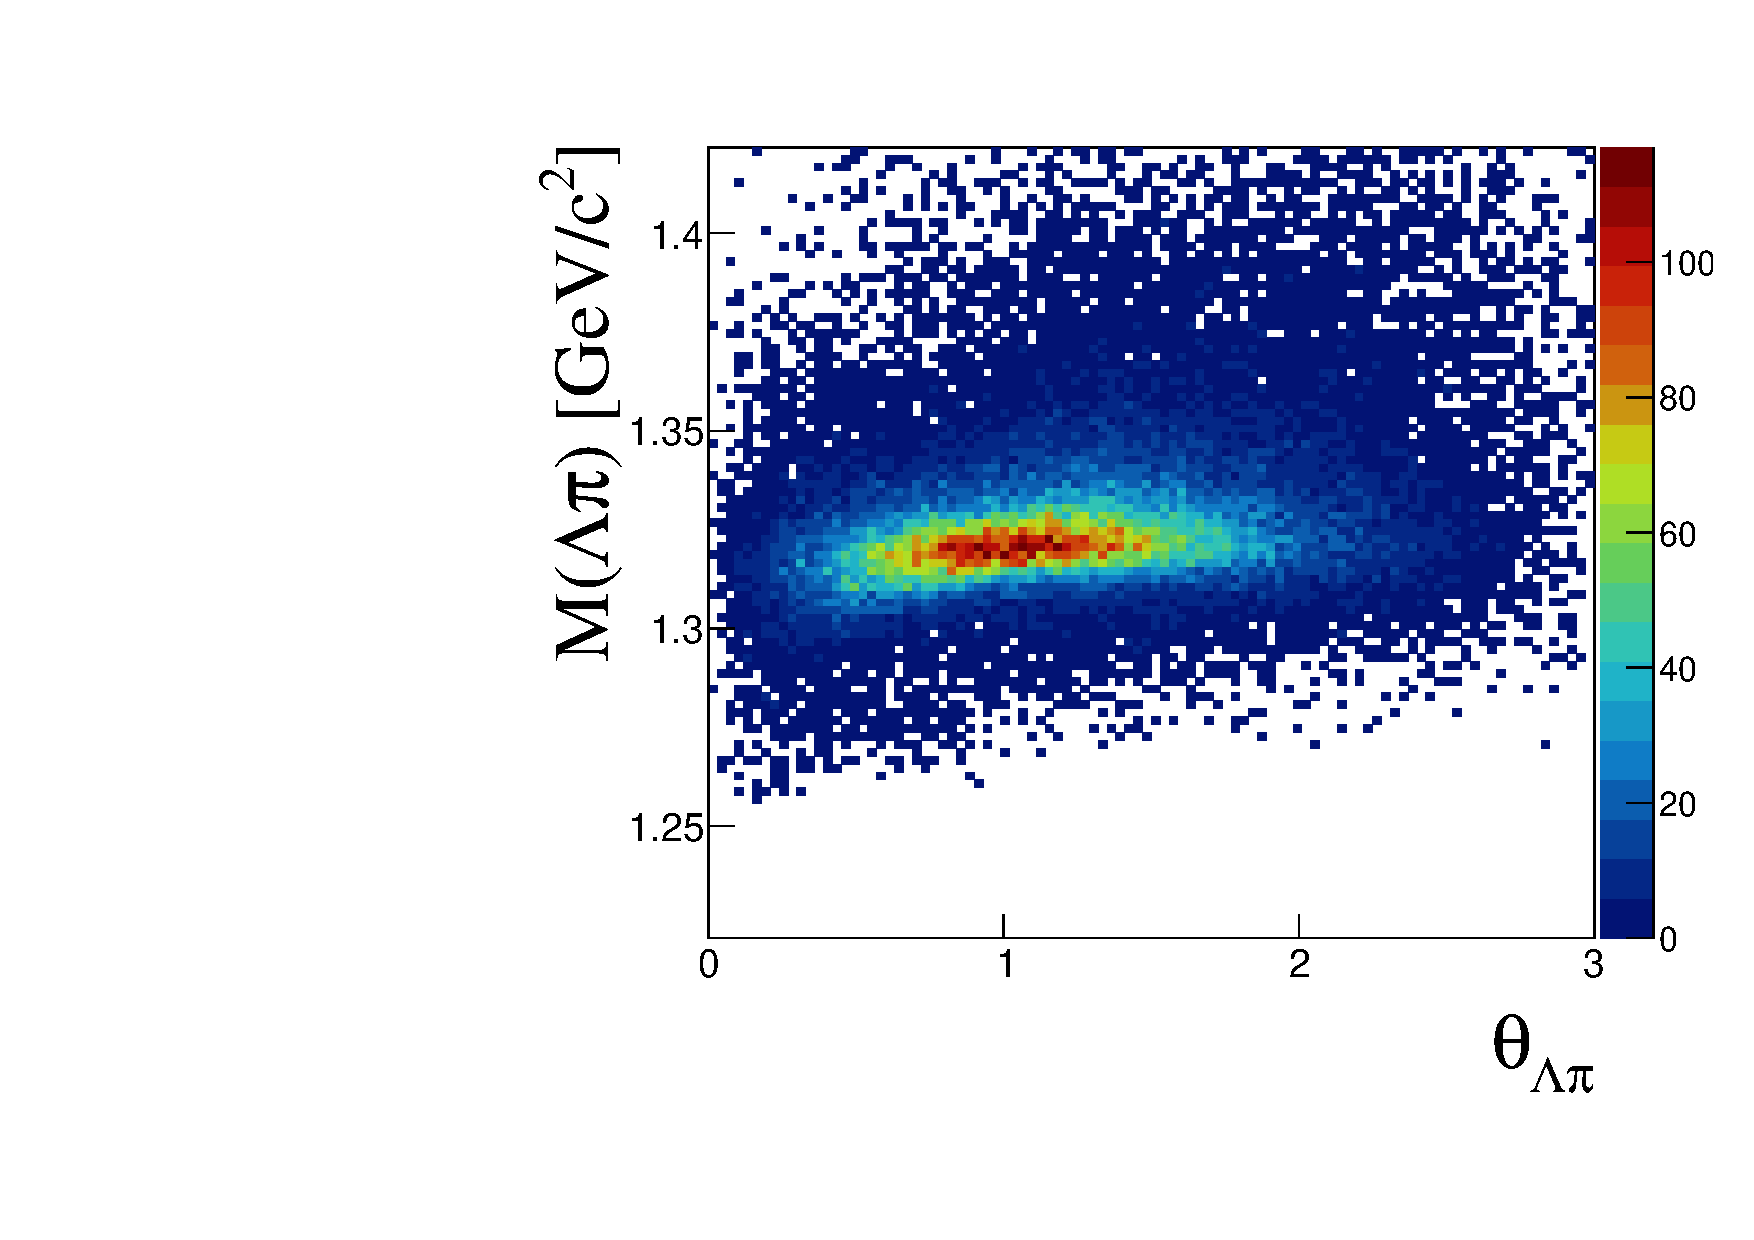
\includegraphics[width=.95\textwidth]{hXiOpening_Mass_CutStandard}}
				\put(30,50){\rotatebox{15}{\Huge\textcolor{tubsgray20}{Preliminary}}}
			\end{picture}		
		\end{figure}
	}{
		\begin{figure}
			\begin{picture}(200,150)
				\put(-10,-30){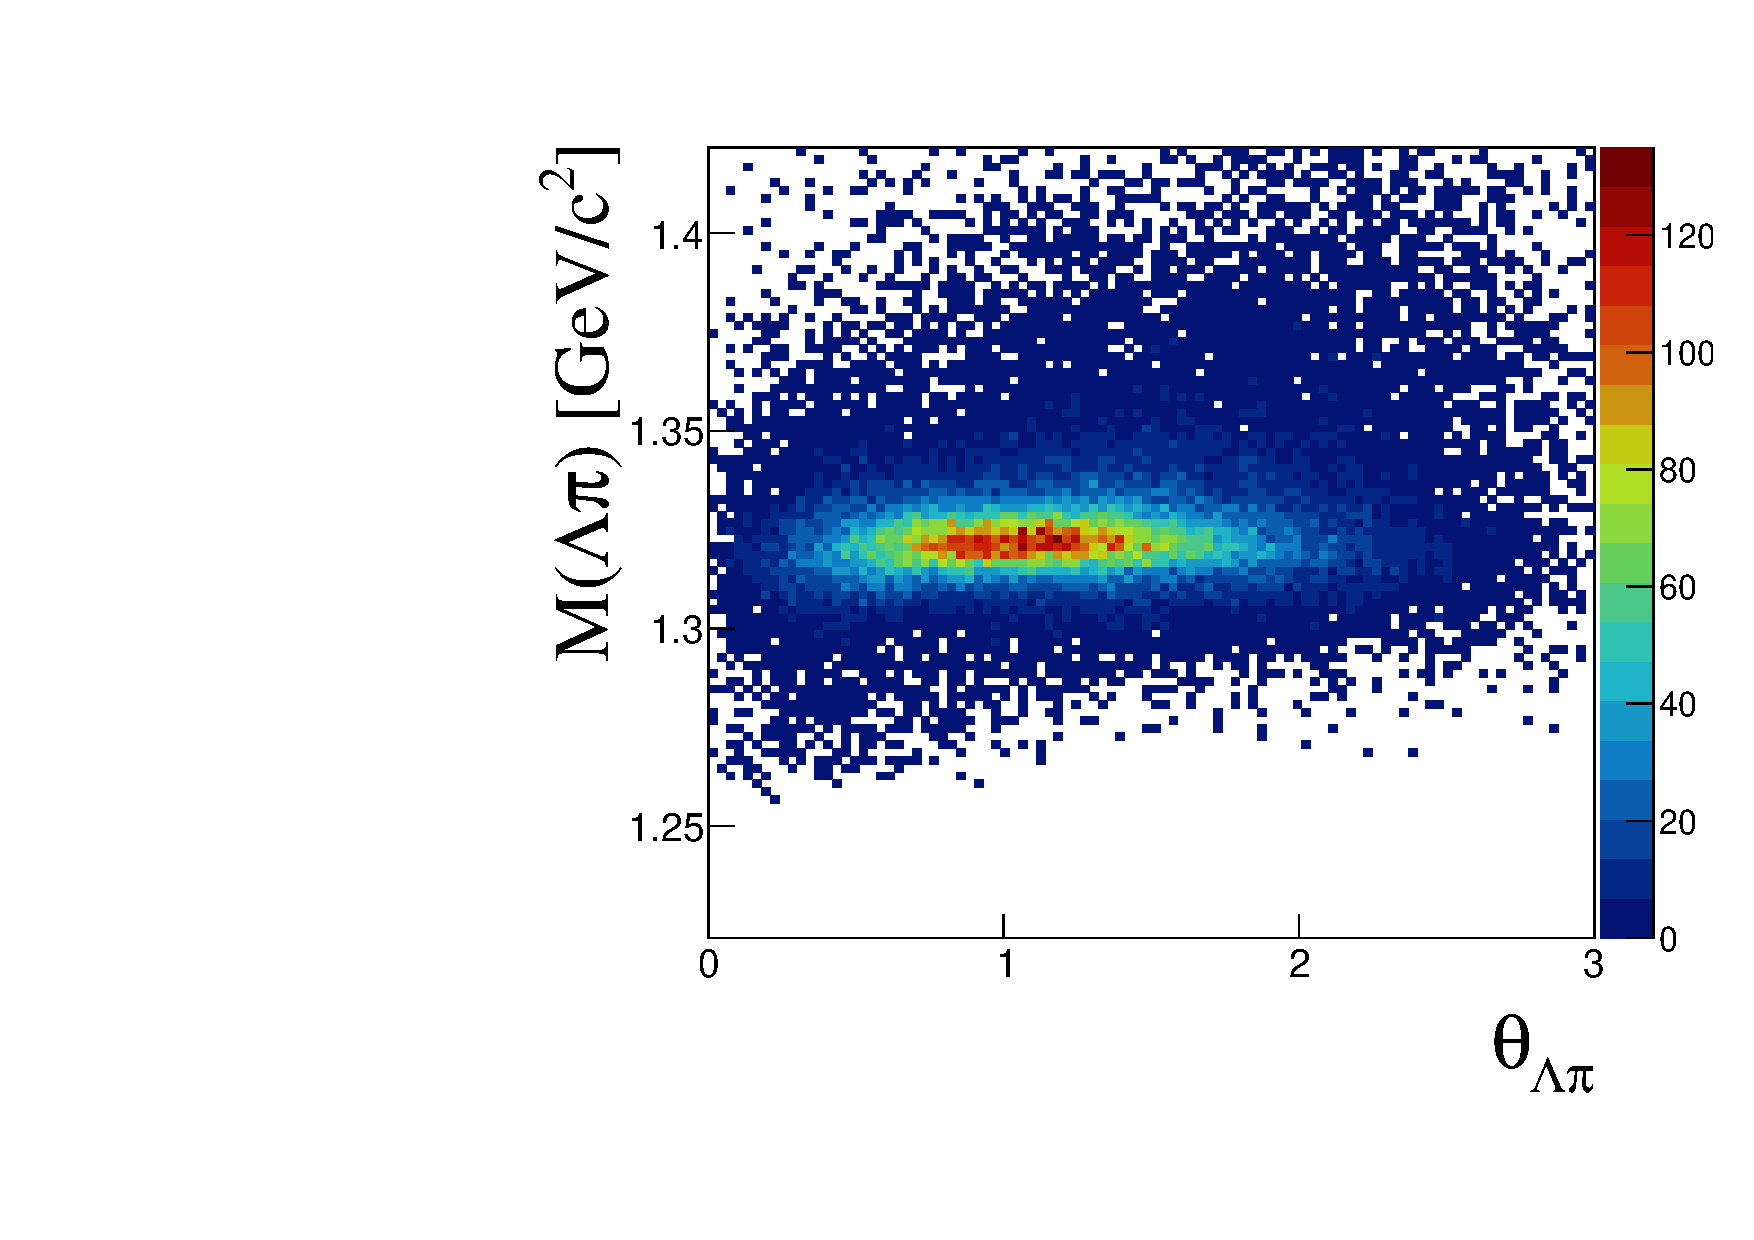
\includegraphics[width=.95\textwidth]{hXiOpening_Mass_CutCor}}
				\put(30,50){\rotatebox{15}{\Huge\textcolor{tubsgray20}{Preliminary}}}
			\end{picture}		
		\end{figure}
	}
\end{frame}
\begin{frame}{Pull distribution}
	\tcl{8}{8}{
		\begin{figure}
			\begin{picture}(200,150)
				\put(0,0){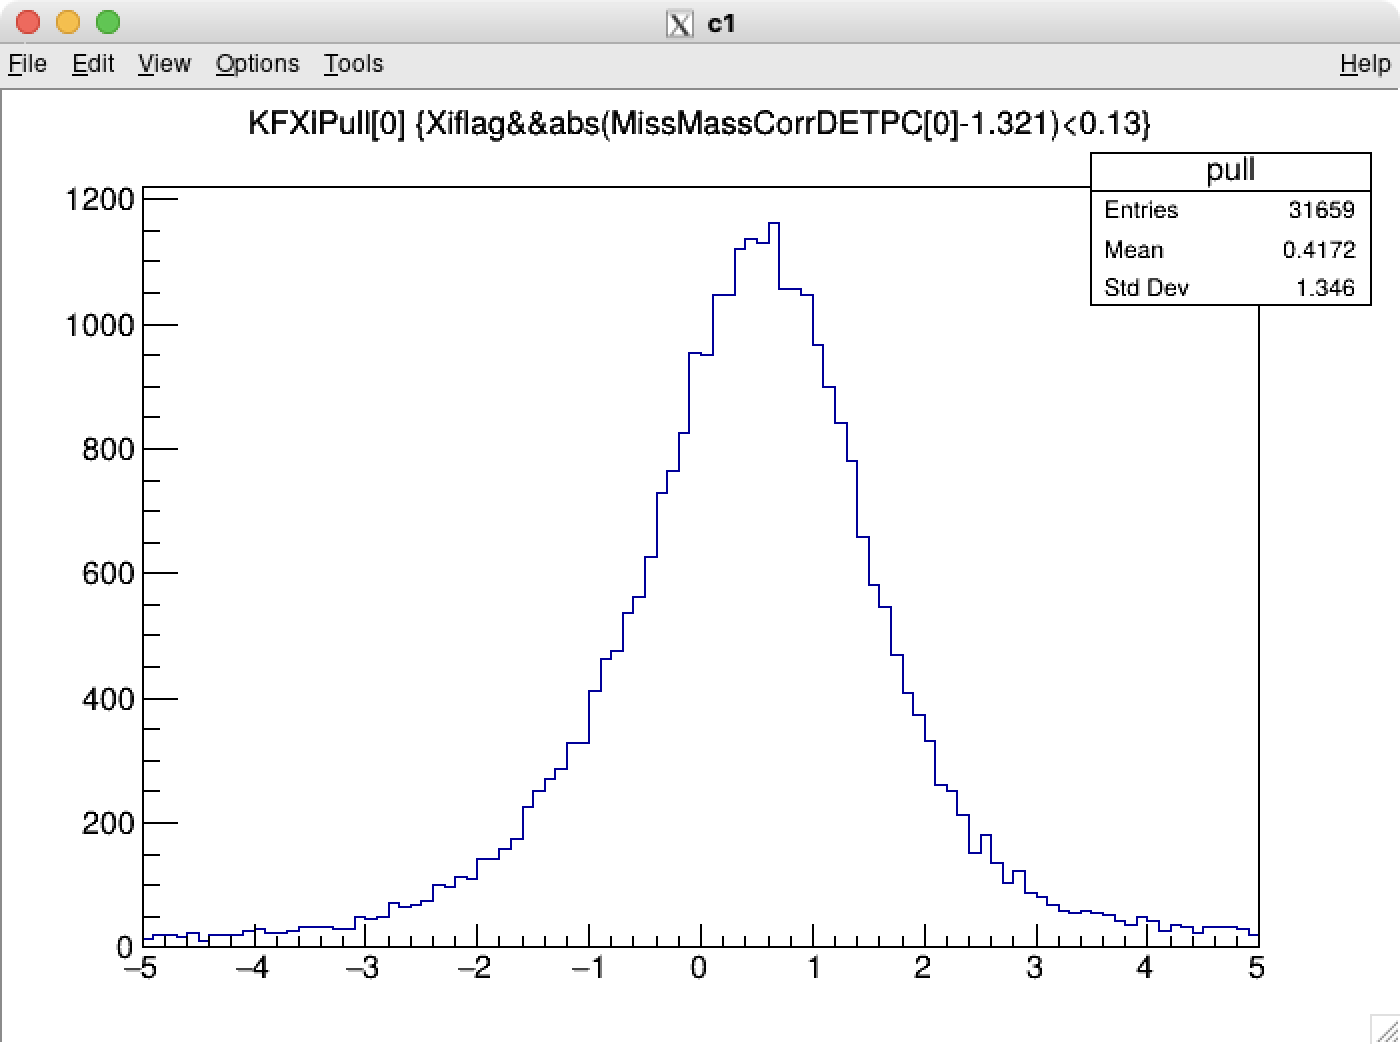
\includegraphics[width=.95\textwidth]{Xi_Pull_Before}}
				\put(30,50){\rotatebox{15}{\Huge\textcolor{tubsgray20}{Preliminary}}}
			\end{picture}		
		\end{figure}
	}{
	\begin{figure}
		\begin{picture}(200,150)
			\put(0,0){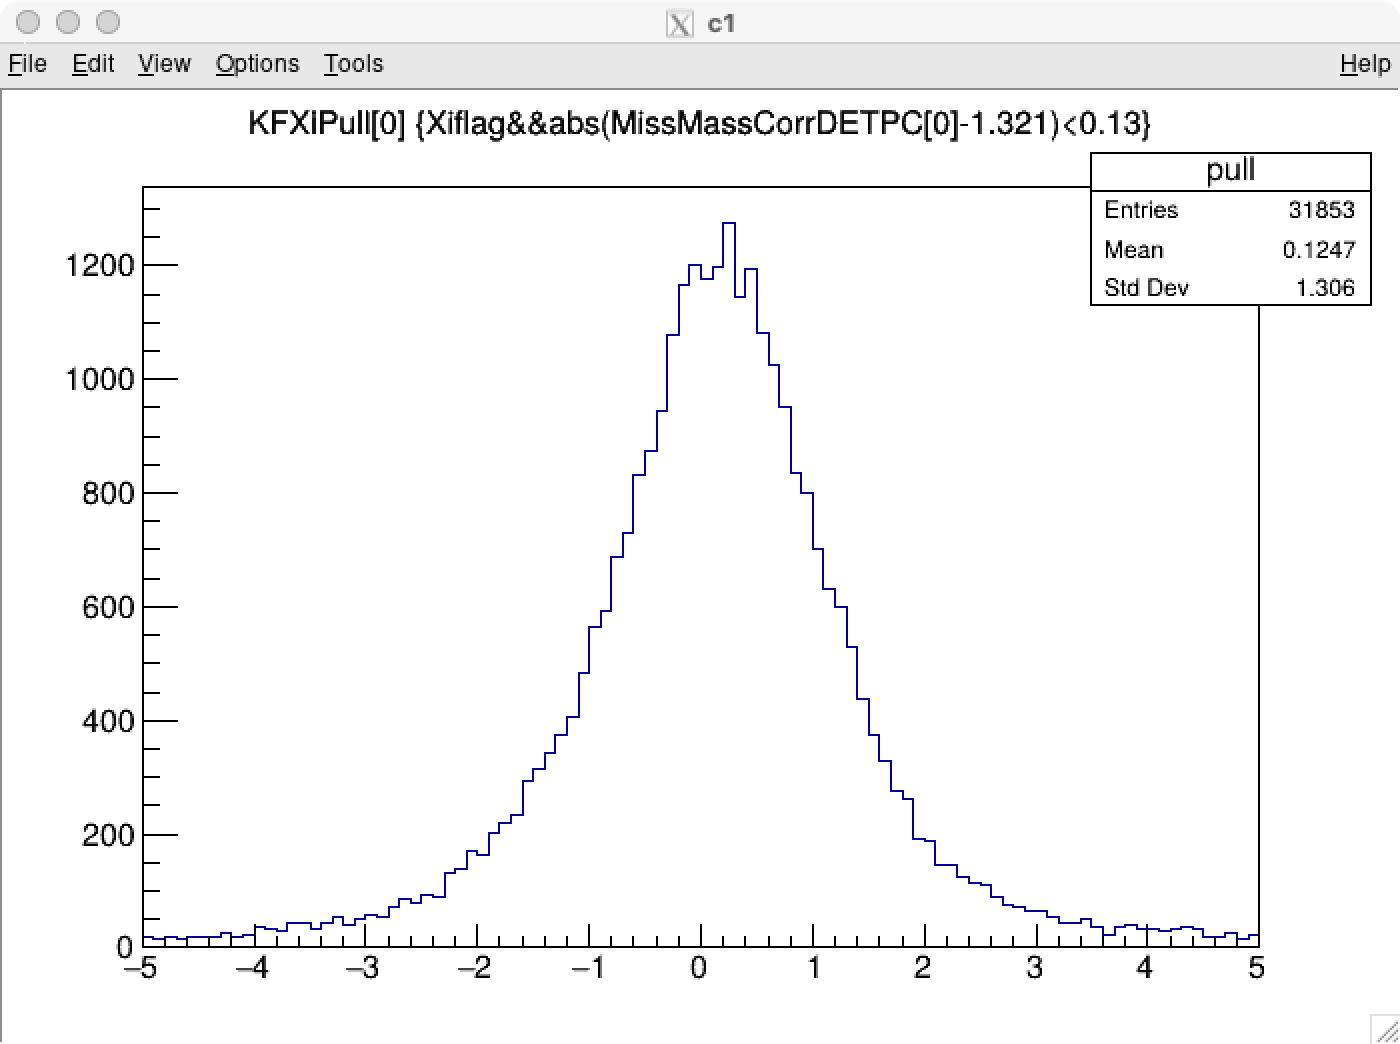
\includegraphics[width=.95\textwidth]{Xi_Pull_After}}
			\put(30,50){\rotatebox{15}{\Huge\textcolor{tubsgray20}{Preliminary}}}
		\end{picture}		
	\end{figure}
	}
\end{frame}

\section{Tricks}
\begin{frame}{Variance Normalization}
	\begin{block}{}
		\begin{align}
			V =
			 \begin{pmatrix}
				10^{12}&0.9\\
				0.9&10^{-12}
			\end{pmatrix}\to V^{-1} = ?
		\end{align}
		While taking an inverse of the variance, matrix elements with different order may be added together, leading to possible numerical unstability. 
		\begin{align}
			\tilde V = S V S^T; S\equiv 
				\frac{1}{\sqrt{V_{ij}}}\delta_{ij}\to \tilde V=\begin{pmatrix}
					1 & Cov(01)/\sigma_{1}\sigma_{2}&\cdots \\
					Cov(01)/\sigma_{1}\sigma_{2}& 1& \\
					\cdots&&\cdots
				\end{pmatrix}
		\end{align}
		We can take out scaling factors in S. Measurement vectors could share the same problem, so they should also be scaled. We rewrite equation \eqref{KFChi2}
		\begin{align}
			\chi^2 = dM^\dagger V^{-1} dM +\cdots= d\tilde M^\dagger \tilde V^{-1}d\tilde M+\cdots;\quad d \tilde M = S(M-M_0) 
		\end{align}
	\end{block}
\end{frame}
\begin{frame}{Off-diagonal Reduction}
	\begin{block}{}
		\begin{align}{}
			V = \begin{pmatrix}
					1&-1\\
					-1&1
			\end{pmatrix}\to V^{-1} = ?
		\end{align}
		Adding off-diagonal term could make matrix uninvertable.  Also we require $\chi^2 = dM V^{-1} dM >0$; $V^{-1}$ (hence V)should be \textit{Positive Definite}. 
		Then, we can 'damp' the offdiagonal elements.
		\begin{align}
			while(IsPositiveDefinite(V))\\
			V_{ij} \to V_{ij}  - \alpha (\delta_{ij}-1) V_{ij}
		\end{align}
		\begin{block}{Property of Positive Definite Matrix}
			All Eigenvalues are Positive! TMatrixD well-supports eigenvalues, so we can just use it.
		\end{block}
	\end{block}
\end{frame}
\begin{frame}{Summary}
	\Large
	\begin{block}{}
		\begin{itemize}
			\item Measurement error can be reduced by correlating the measurements with physical constraints; This process is Kinematic Fit.
			\item By observing statistical parameters, we can estimate many physical context other than error reduction.(i.e. Resolution/Bias estimation, S/N separation, etc...)
			\item Proper understandings of covariance matrix is required for Kinematic Fit.
		\end{itemize}
	\end{block}
	
\end{frame}
\section{Appendix}
\begin{frame}{Minimization Steps.}
	\large
	\begin{block}{}
		The coupled differential equations \eqref{GradM},\eqref{GradL} and \eqref{GradU} will be solved iteratively. For each $\nu$th step,
		\begin{align}
			&V^{-1}(\mathbf m^0)(\mathbf{m}^{\nu+1}-\mathbf{m}^0)+(\mathbf{F}_m^\dagger)^\nu\mathbf\lambda^{\nu+1}=0\label{DelM}\\
			&(\mathbf{F}_u^\dagger)^\nu\mathbf\lambda^{\nu+1}=0\label{DelL}\\
			&\mathbf f^\nu + \mathbf F^\nu_m (\mathbf m^{\nu+1}-\mathbf m^\nu) + \mathbf F^\nu_u(\mathbf u^{\nu+1}-\mathbf u^\nu)=0\label{DelU}.
		\end{align}
		Equation \eqref{DelU} is not a direct consequence of Equation \eqref{GradU} but rather a \textit{linear approximation}.  
		
		Note that, as we are determining the parameters $\mathbf m, \mathbf u$ and $\mathbf \lambda$, they are indexed as $\nu+1$, while constraint terms(i.e. $\mathbf f,\mathbf F_\mu$ and $\mathbf F_\nu$) are calculated from current step, $\nu$. This fit is basically using Newton's method.
	\end{block}
\end{frame}

\begin{frame}{Coupled Equation Solving (1)}
	\begin{block}{}
		Multiplying \textbf V to Equation \eqref{DelM} leads to:	
		\begin{align}
			\mathbf{m}^{\nu+1}-\mathbf{m}^0=-V(\mathbf m^0)(\mathbf{F}_m^\dagger)^\nu\mathbf\lambda^{\nu+1}.\label{Mnu}
		\end{align}
		Substituting Equation \eqref{Mnu} into Equation \eqref{DelU}, 
		\begin{align}
			\mathbf F^\nu_u(\mathbf u^{\nu+1}-\mathbf u^\nu) &= - \mathbf f^\nu - \mathbf F^\nu_m (-V(\mathbf m^0)(\mathbf{F}_m^\dagger)^\nu\mathbf\lambda^{\nu+1} +\mathbf{m}^0-\mathbf{m}^\nu  )\nonumber\\
			&=  S\lambda^{\nu+1}  - R\label{SLambda}
		\end{align}
		where we define the \textit{constraiint covariance} $S$ and \textit{residual} $R$ as:
		\begin{align}
		S\equiv \mathbf{F}_\mathbf{m}^\nu V(\mathbf m^0)(\mathbf{F}_\mathbf{m}^\dagger )^\nu;\quad R\equiv \mathbf f^\nu + \mathbf{F}_\mathbf{m}^\nu(\mathbf{m}^0-\mathbf{m}^\nu)
		\end{align}
		  Multiplying $(\mathbf{F}_u^\dagger)^\nu S^{-1}$  into \eqref{SLambda}, we get:
		\begin{align}
			(\mathbf{F}_u^\dagger)^\nu S^{-1}\mathbf F^\nu_u(\mathbf u^{\nu+1}-\mathbf u^\nu) = \cancelto{0,\because \eqref{DelL}}{(\mathbf F_u^\dagger)^\nu\mathbf \lambda^{\nu+1}}-(\mathbf{F}_u^\dagger)^\nu S^{-1}R.
		\end{align}
	\end{block}
\end{frame}
\begin{frame}{Coupled Equation Solving (2)}
	\begin{block}{}
		Then we naturally derive the expressions
		\begin{align}
			\mathbf{u}^{\nu+1}=\mathbf{u}^\nu - ((\mathbf{F}_u^\dagger)^\nu S^{-1}\mathbf F^\nu_u)^{-1}(\mathbf{F}_u^\dagger)^\nu S^{-1}R\label{Unu}.
		\end{align} 
		and from \eqref{SLambda},
		\begin{align}
			\mathbf\lambda^{\nu+1} = S^{-1}(\mathbf F^\nu_u(\mathbf u^{\nu+1}-\mathbf u^\nu) + R)\label{Lnu}.
		\end{align}
		For a summary, we have obtained all equations to proceed to the next step. All other matrices in the equation can be calculated from parameters of the current step, and $\chi^2$ can be evaluated from \eqref{KFChi2} .
		\begin{align*}
			\begin{cases}
				\mathbf{u}^{\nu+1}=\mathbf{u}^\nu - ((\mathbf{F}_u^\dagger)^\nu S^{-1}\mathbf F^\nu_u)^{-1}(\mathbf{F}_u^\dagger)^\nu S^{-1}R&\eqref{Unu}\\
				\mathbf\lambda^{\nu+1} = S^{-1}(\mathbf F^\nu_u(\mathbf u^{\nu+1}-\mathbf u^\nu) + R)&\eqref{Lnu}\\
				\mathbf{m}^{\nu+1}=\mathbf{m}^0-V(\mathbf m^0)(\mathbf{F}_m^\dagger)^\nu\mathbf\lambda^{\nu+1}&\eqref{Mnu}
			\end{cases}
		\end{align*}
	\end{block}
\end{frame}
\begin{frame}{Covariance Matrix Propagation}
	\begin{block}{}
		We estimate the covariance for the fitted variables, $m$,
		\begin{align}
			V(m) = J_{m,m^0}V(m^0)J_{m,m^0}^\dagger\label{VarianceEvolve}
		\end{align}
		To solve \eqref{VarianceEvolve} the Jacobian should be determined.
		\begin{align}
			J_{m,m^0(i,j)} = \pdf{m_i}{m^0_j}\label{Jacobian}
		\end{align}
	\end{block}
\end{frame}
\begin{frame}{Jacobian}
	\begin{block}{}
		To begin with, let us express Eq \eqref{Mnu} in terms of $m^0$. At the moment we will drop the superscript $\nu$. As $\vecb f(\vecb m,\vecb u)$is a constant on $m^0$, $\vecb F_\vecb m$ also will be a constant to $m^0$. Then we only need to consider the derivatives of $\lambda$. By substituting \eqref{Unu} ,
		\begin{align}
	\mathbf\lambda = S^{-1}(-\mathbf F_u(((\mathbf{F}_u^\dagger) S^{-1}\mathbf F_u)^{-1}(\mathbf{F}_u^\dagger) S^{-1}R) + R)
		\end{align}
		and the residual matrix is:
		\begin{align}
			R\equiv \mathbf f + \mathbf{F}_\mathbf{m}(\mathbf{m}^0-\mathbf{m})\to \pdf{R}{m^0}= \vecb F_m
		\end{align} 
		Now we obtain the derivative of $\lambda$ as:
		\begin{align}
			\pdf{\lambda}{m^0}= S^{-1}(-\mathbf F_u((\mathbf{F}_u^\dagger S^{-1}\mathbf F_u)^{-1}\mathbf{F}_u^\dagger S^{-1}\vecb F_m) + \vecb F_m).
		\end{align}
	\end{block}
\end{frame}
\begin{frame}{Jacobian}
	\begin{block}{}
		Now define the symmetric matrices
		\begin{align}
			G\equiv \vecb {F_m^\dagger} S^{-1}\vecb {F_m};\quad U\equiv (\mathbf{F}_u^\dagger S^{-1}\mathbf F_u)^{-1};\quad H\equiv \mathbf{F}_m^\dagger S^{-1}\vecb {F_u}
		\end{align}
		We have expressions for $\pdf{\lambda}{m^0}$. Equation \eqref{Jacobian} is determined as:
		\begin{align}
			J_{m,m^0}&=I - V(m^0)\vecb{F}_m^\dagger\pdf\lambda{m^0}=I - V\vecb{F}^\dagger_m(-S^{-1}\vecb F_u U^{-1}H^\dagger+S^{-1}\vecb F_m)\nonumber\\
			&=I-V(G-HUH^\dagger)
		\end{align}
		If we let $C =G-HUH^\dagger$, we obtain
		\begin{align}
			V(m) = J_{m,m^0} VJ_{m,m^0}^\dagger =V -2 VCV  +VCVCV.\label{Vm}
		\end{align}
		We would keep 2nd order term at the moment. Some materials like \cite{Prob} had an error in this part.
	\end{block}
\end{frame}

\begin{frame}{Variance of the Unknowns}
	\begin{block}{}
		Just like how we derived  Eq.\eqref{Vm} we can estimate the variance matrix of the unknowns. 
		\begin{align}
			V_U = J_{u,m0} V J_{u,m0}^T
		\end{align}
		$J_{u,m0}$ can be obtained from Eq.\eqref{Unu}. Defining 
		\begin{align}
			K\equiv ((\mathbf{F}_u^\dagger)^\nu S^{-1}\mathbf F^\nu_u)^{-1}(\mathbf{F}_u^\dagger)^\nu S^{-1}
		\end{align}
		we write:
		\begin{align}
			J_{u^{\nu+1},m^0} = \pdf {u^{\nu+1}} {m^0} = \pdf{u^{\nu}}{m^0} - K\pdf R {m^0} \simeq -K \vecb F_m.
		\end{align}
		Note that we only have initial "Guess" for the unknowns; In principle, it is not a driven value from measurements. Then, $\pdf {u^0}{m_0} = 0$. Also, we approximate that the terms in 2nd or higher iterations are negligible: $J_{u,m^0}\simeq J_{u^0,m^0}$.
	\end{block}
\end{frame}
\begin{frame}{Pull distribution}
	\begin{block}{}
		The covariance in Equation \eqref{Ve} is estimated as:
		\begin{align}
			Cov(m,m^0) = J_{m,m^0}V(m) = V - VCV.
		\end{align}
		If we substitute this and Eq.\eqref{Vm} into Eq.\eqref{Ve}, we get
		\begin{align}
			V(\epsilon) = VCVCV.
		\end{align}
		Note that 2nd order term affects the covariance matrix of the correction. 
	\end{block}
\end{frame}
\begin{frame}{KinFit Package}
	\tcl{8}{8}{
		\begin{figure}
			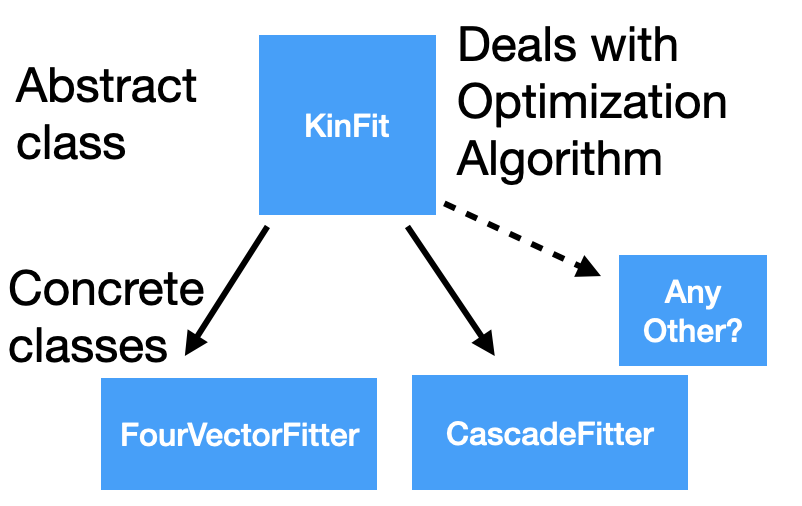
\includegraphics[width=.9\textwidth]{KinFit}
		\end{figure}
	}{
		\large
		\begin{align}
			\chi^2 = \delta M^T V^{-1}\delta M + 2\lambda f(M,U)
		\end{align}
		\vspace{-5 mm}
		\begin{block}{KinFIt provides...}
			\begin{itemize}
				\item Minimize $\chi^2$
				\item Calculate pulls and p-values
			\end{itemize}
		\end{block}
		\begin{block}{Users should...}
			\begin{itemize}
				\item Assign proper variables for M and U
				\item Define physical constraints
				\item Write the derivatives, $F_M$ and $F_U$ by hand
			\end{itemize}
		\end{block}
	}
\end{frame}
%\begin{frame}[allowframebreaks]{References}
\begin{frame}{References}
	 	\printbibliography
\end{frame}
\end{document}
